\documentclass[a4paper,12pt]{scrartcl}

\usepackage{graphicx}


\usepackage[ngerman] {babel}
\usepackage[T1]{fontenc}
\usepackage{float}
\usepackage[utf8]{inputenc}
\usepackage{fancyhdr}
\pagestyle{fancy}
\usepackage{subfigure} 


\lhead{1}
\chead{2}
\rhead{3}

\lfoot{4}
\cfoot{5}
\rfoot{6}


\setlength{\parindent}{0em} 

\title{Diplomarbeit}
\author{Dominik Pichler}
\date{21. Jänner 2018}

\begin{document}

\maketitle
\setcounter{tocdepth}{5}
\setcounter{secnumdepth}{4}
\tableofcontents

\section{Teil 1 Mechanik}
\subsection{Einleitung}
\subsection{Aufgabenstellung}
\subsubsection{Zielsetzung}
\subsubsection{Problematik}
\newpage
\subsection{Konzepte} 



\subsubsection{Variante 1} 
\textbf{Übersicht der Prozessschritte:}
\begin{itemize}
\item[1] Füllen des Futtermagazins
\item[2] Führen zur Schneidplatte
\item[3] Schnitt
\item[4] Pressen
\item[5] Entsorgen
\item[6] Füttern
\end{itemize}

\paragraph{Füllen des Futtermagazins}$~~$\\

Im folgenden Bild wird mithilfe einer Lego-Darstellung gezeigt, wie das Magazin aus verschiedenen Blickwinkeln befüllt aussieht. Hier muss man beachten das die vom Hersteller zu öffneten Seite in Richtung des Schneidewerks zeigt (die schmale Seite mit der Einkerbung).

\begin{figure}[H]
\begin{center}
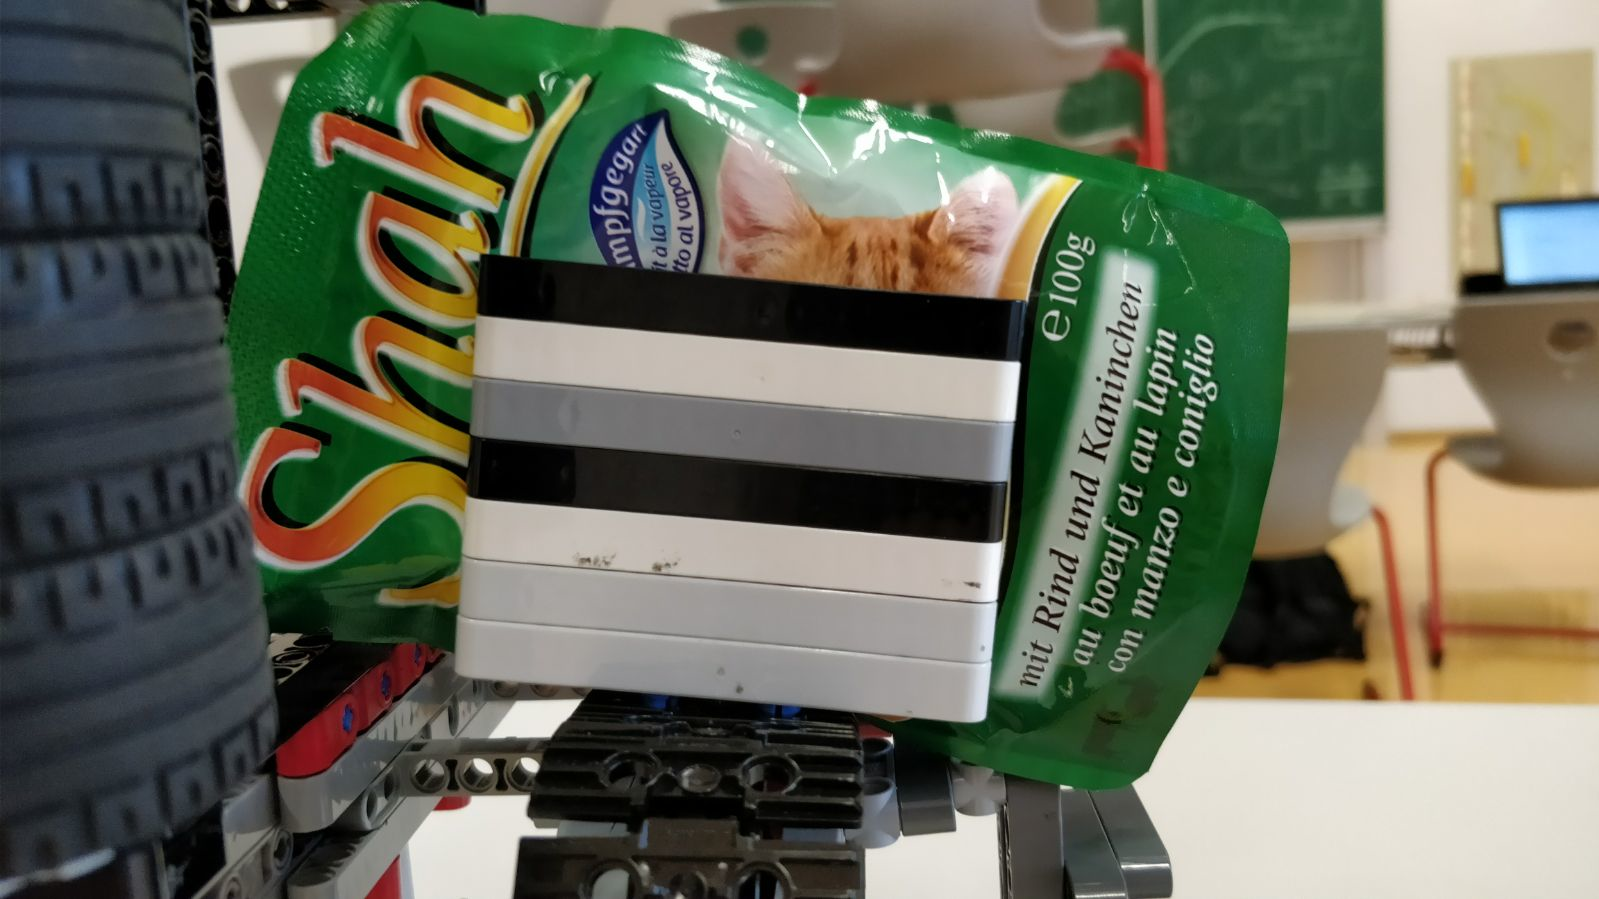
\includegraphics[width=13cm]{Bilder/Ablauf_1_png/Magazin_Vorne.png}
\caption{Magazin Vorne}
\end{center}
\end{figure}

\begin{figure}[H]
\begin{center}
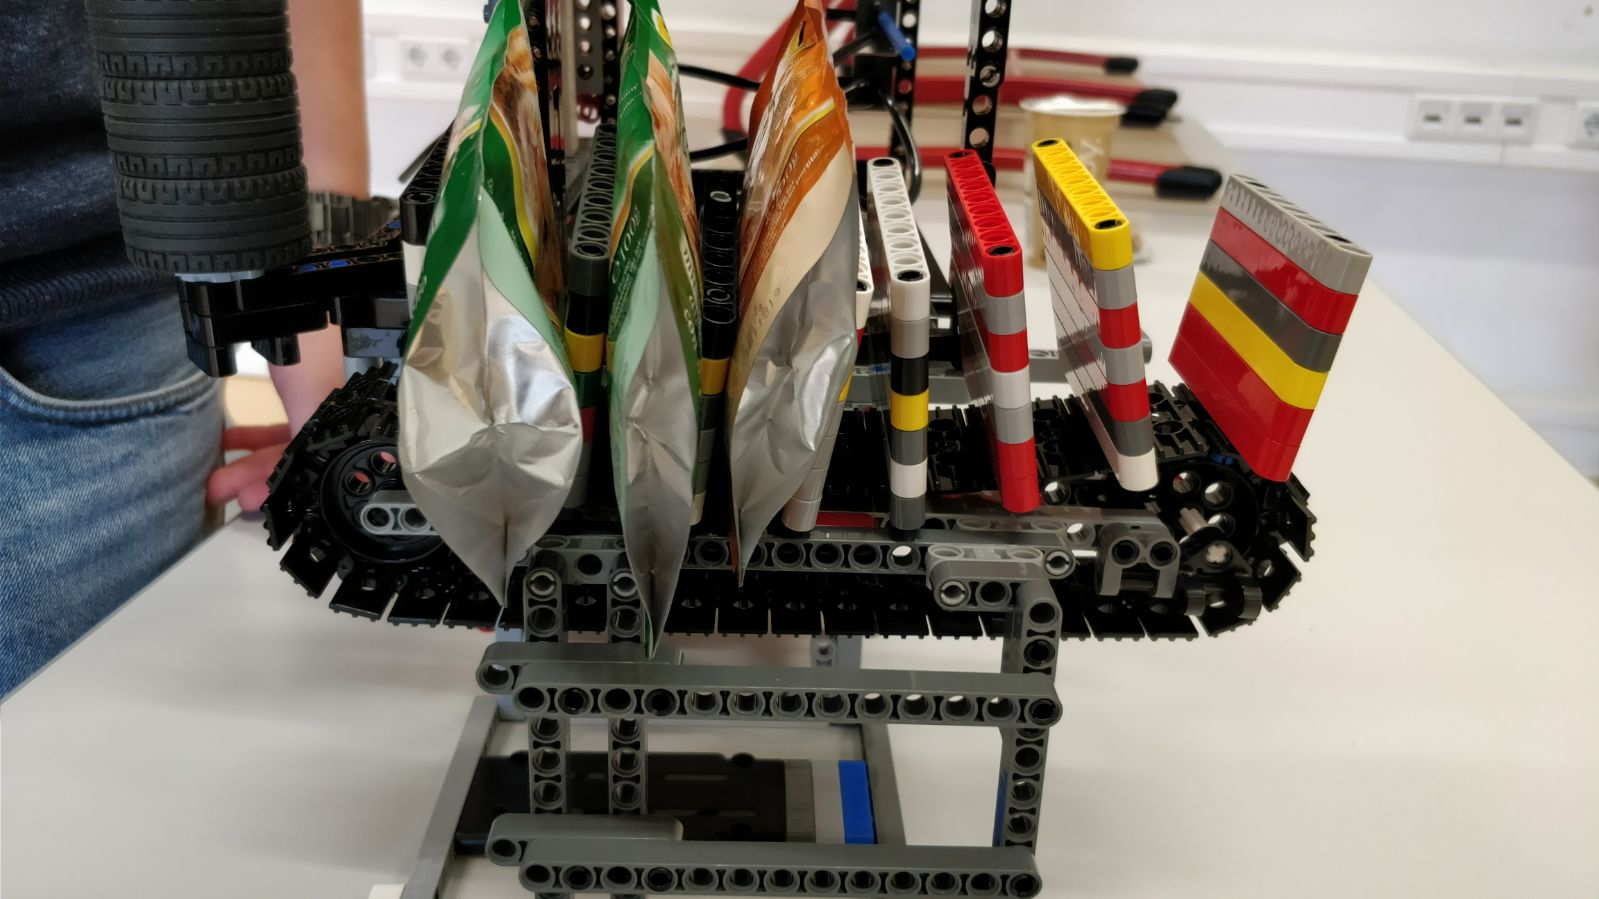
\includegraphics[width=13cm]{Bilder/Ablauf_1_png/Magazin_Seitlich.png}
\caption{Magazin Seitlich}
\end{center}
\end{figure}

\begin{figure}[H]
\begin{center}
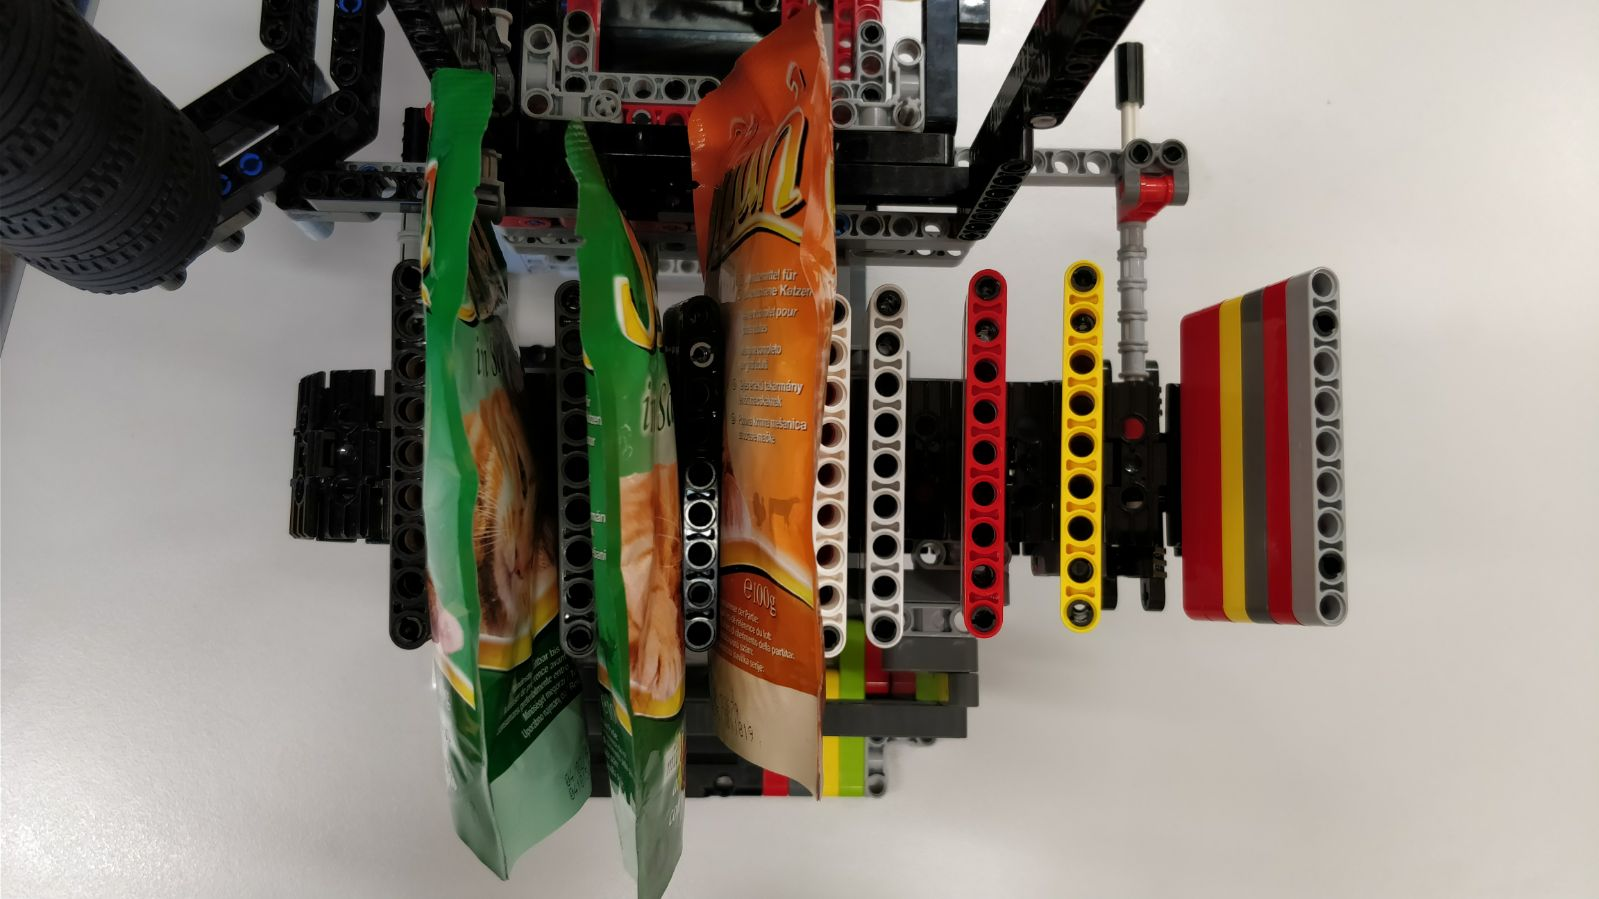
\includegraphics[width=13cm]{Bilder/Ablauf_1_png/Magazin_Oben.jpeg}
\caption{Magazin Oben}
\end{center}
\end{figure}

\newpage 

\paragraph{Führen zur Schneidplatte}$~~$\\  

In diesem Schritt wird mithilfe eines Greifers (dargestellt durch eine Hand) die Packung in richtiger Position gebracht.

\begin{figure}[H]
\begin{center}
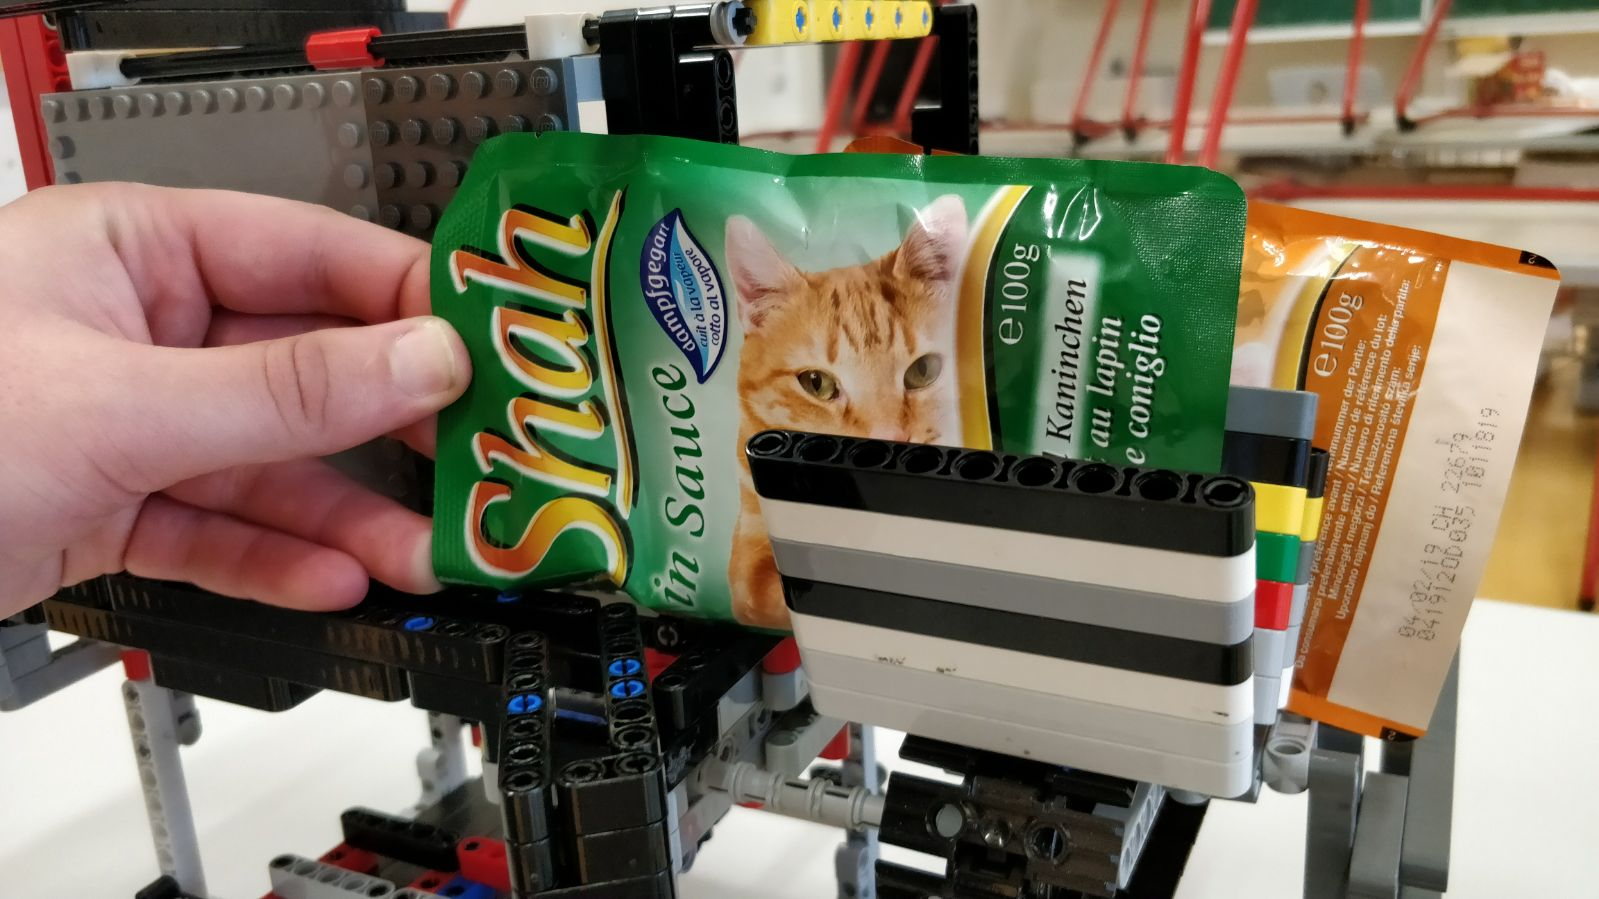
\includegraphics[width=13cm]{Bilder/Ablauf_1_png/Magazin_Auszug.jpeg}
\caption{Magazin Auszug}
\end{center}
\end{figure}

\begin{figure}[H]
\begin{center}
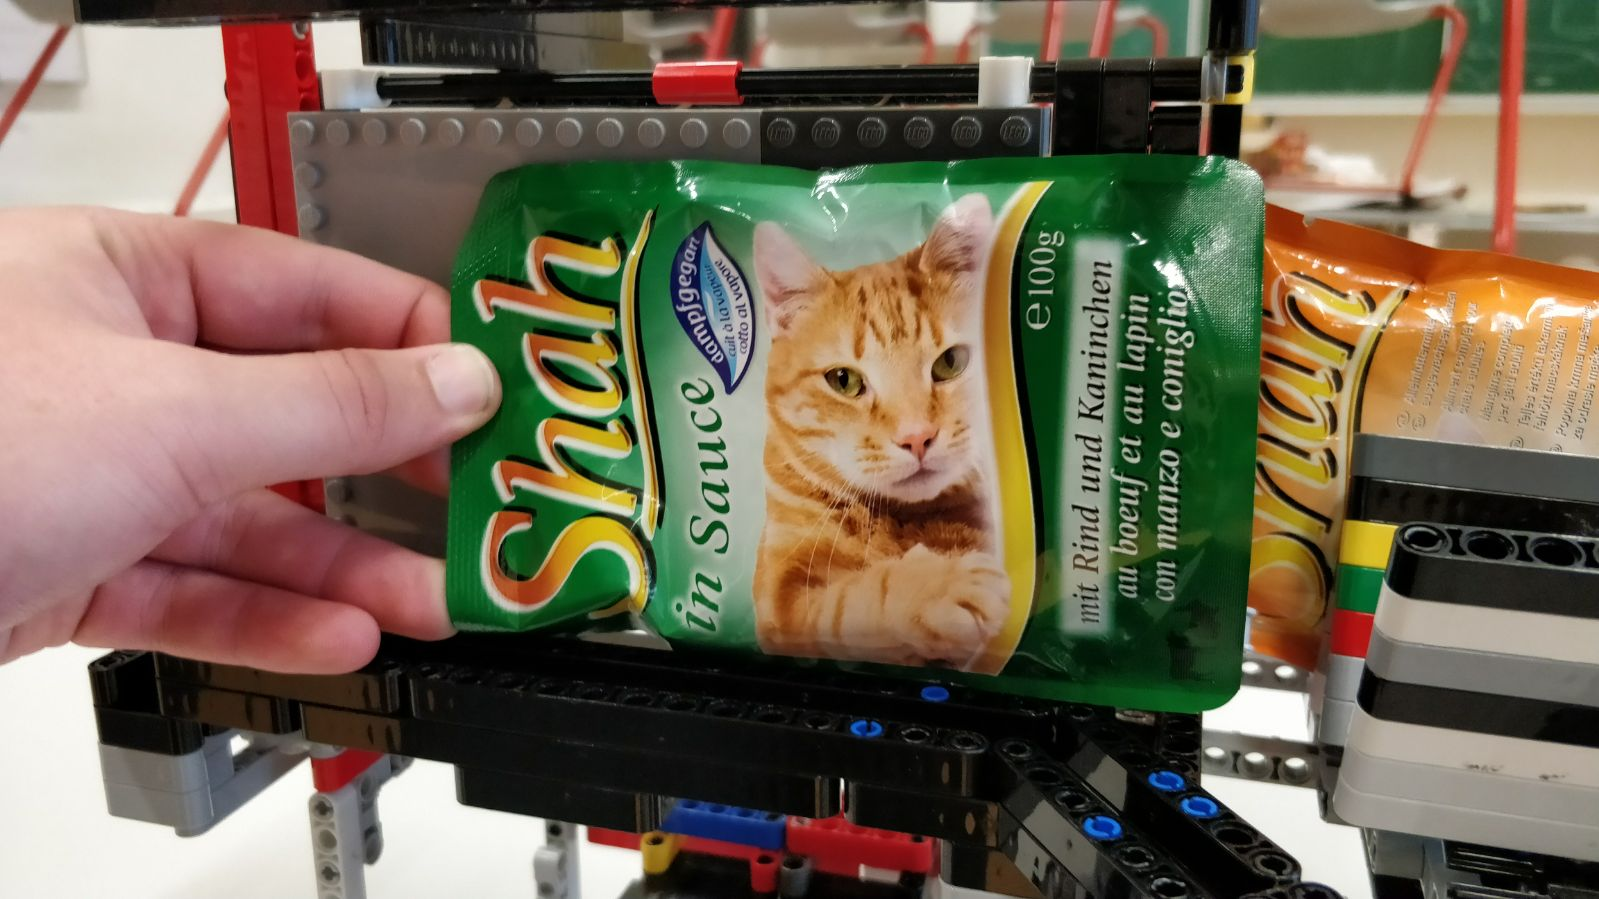
\includegraphics[width=13cm]{Bilder/Ablauf_1_png/Magazin_Auszug_2.jpeg}
\caption{Magazin Auszug 2}
\end{center}
\end{figure}

Wie im Bild gezeigt liegt das Katzenfutterpackerl in der richtigen Position und wird mit zwei Magnetzylindern an der Schneidefläche festgehalten.

\begin{figure}[H]
\begin{center}
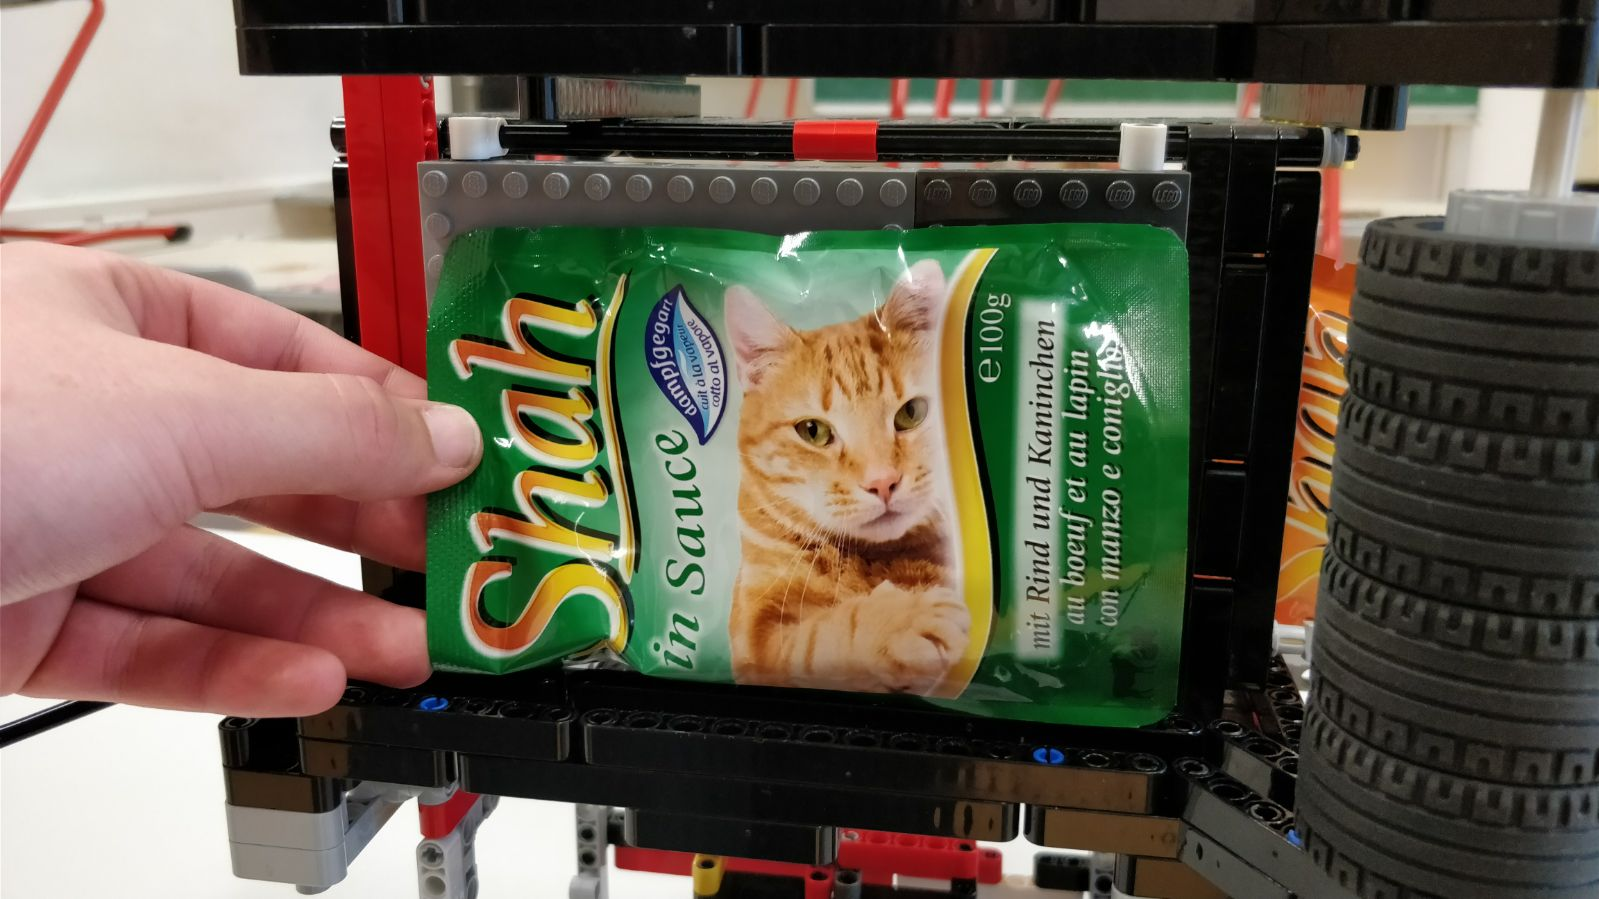
\includegraphics[width=13cm]{Bilder/Ablauf_1_png/Schneidebereit.jpeg}
\caption{Schneidebereit}
\end{center}
\end{figure}

Endposition des Greifers. Kerbe liegt genau an der richtigen Position. 4 Magnetzylinder halten den Futterbeutel and dieser Position, damit der Beutel während des Schneidens nicht verrutscht.

\begin{figure}[H]
\begin{center}
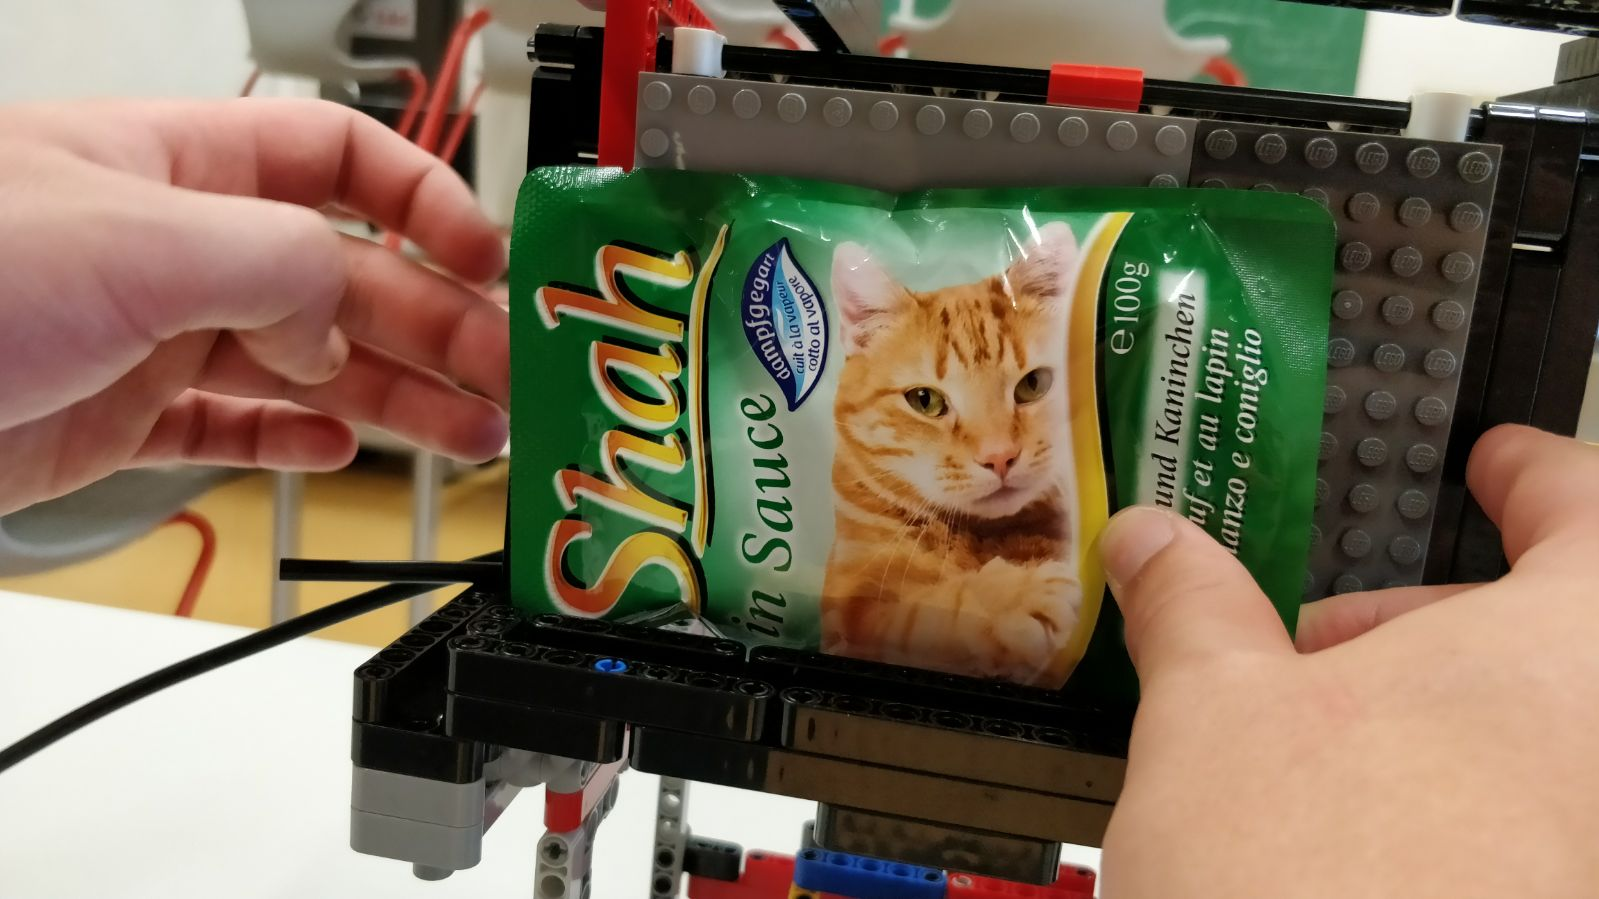
\includegraphics[width=13cm]{Bilder/Ablauf_1_png/Fertig_Geschnitten}
\caption{Fertig Geschnitten}
\end{center}
\end{figure}

\newpage
\paragraph{Schnitt}$~~$\\

In der richtigen Position muss man mit 2 scharfen Klinge mit viel Druck die Packung aufschneiden. Eine davon wird and der Schnittfläche angebracht und die andere macht die Schneidbewegung, wobei die beiden aneinander reibenden Kanten in einem Schnitt resultieren. Die Packung kann mit einem Schnitt vollständig geöffnet werden.

Anhand dieses Bildes wird gezeigt wie der Schnitt funktionieren kann.

\begin{figure}[H]
\begin{center}
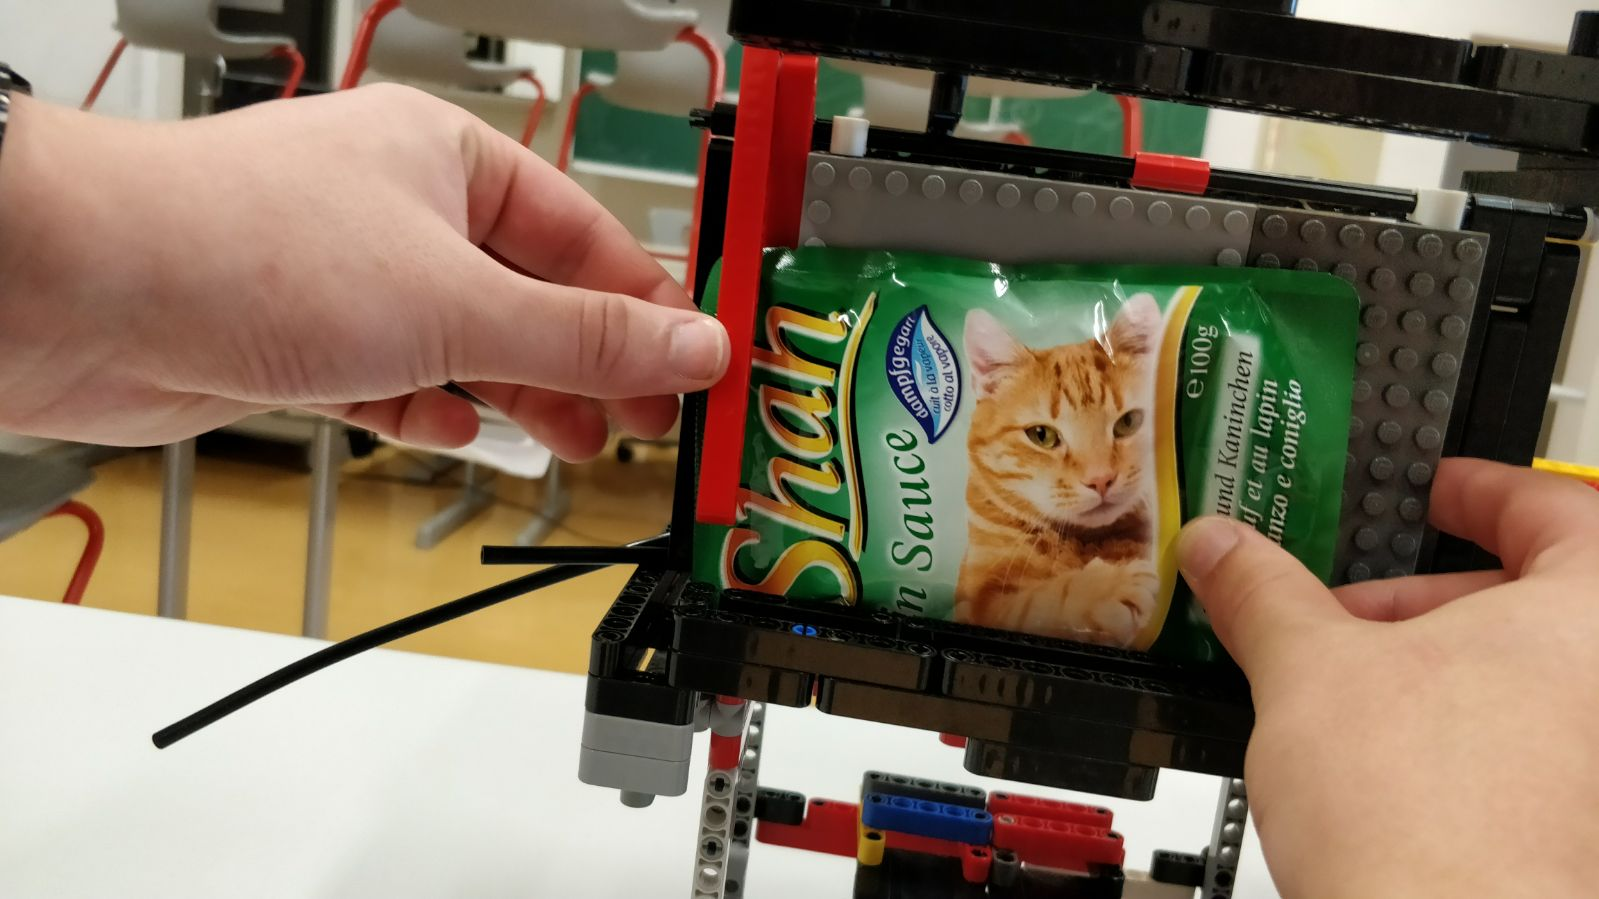
\includegraphics[width=13cm]{Bilder/Ablauf_1_png/Schnitt}
\caption{Schnitt}
\end{center}
\end{figure} 

\newpage
\paragraph{Pressen}$~~$\\

Nach dem Aufschneiden wird mit einer Rolle das Sackerl ausgepresst. Dazu werden zuerst die ersten 2 Magnetzylinder gelöst bis die Rolle vorbei ist. Danach werden sie wieder in Position gebracht. Daraufhin werden die anderen beiden gelöst und die Rolle fährt ans Ende.

\begin{figure}[H]
\begin{center}
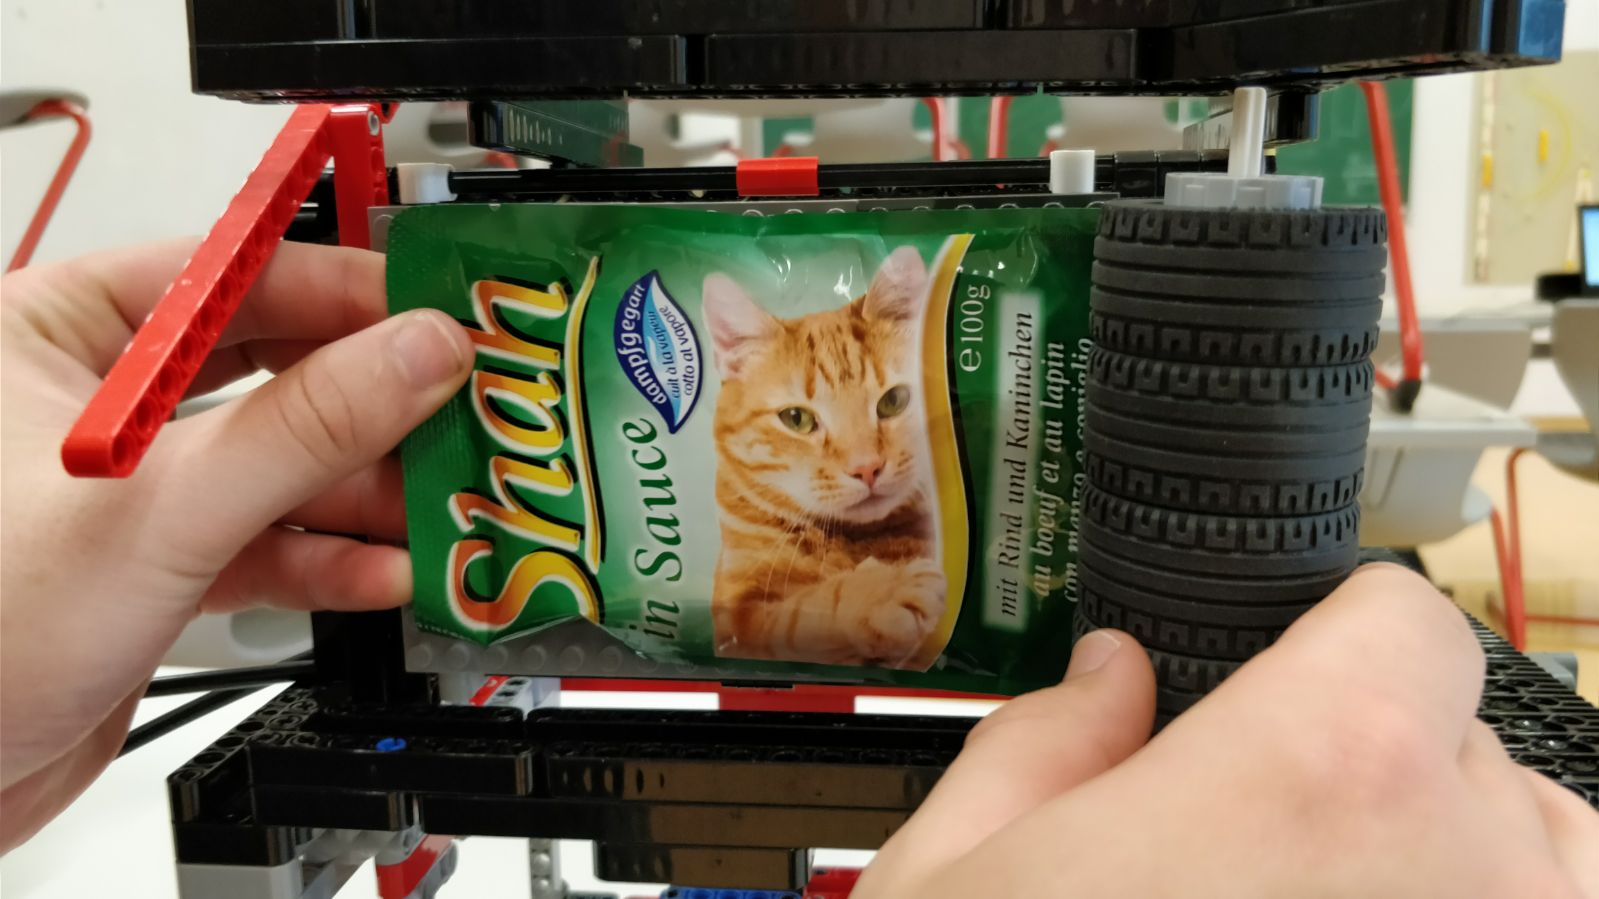
\includegraphics[width=13cm]{Bilder/Ablauf_1_png/Ausquetschen_1}
\caption{Ausquetschen Beginn}
\end{center}
\end{figure}

\begin{figure}[H]
\begin{center}
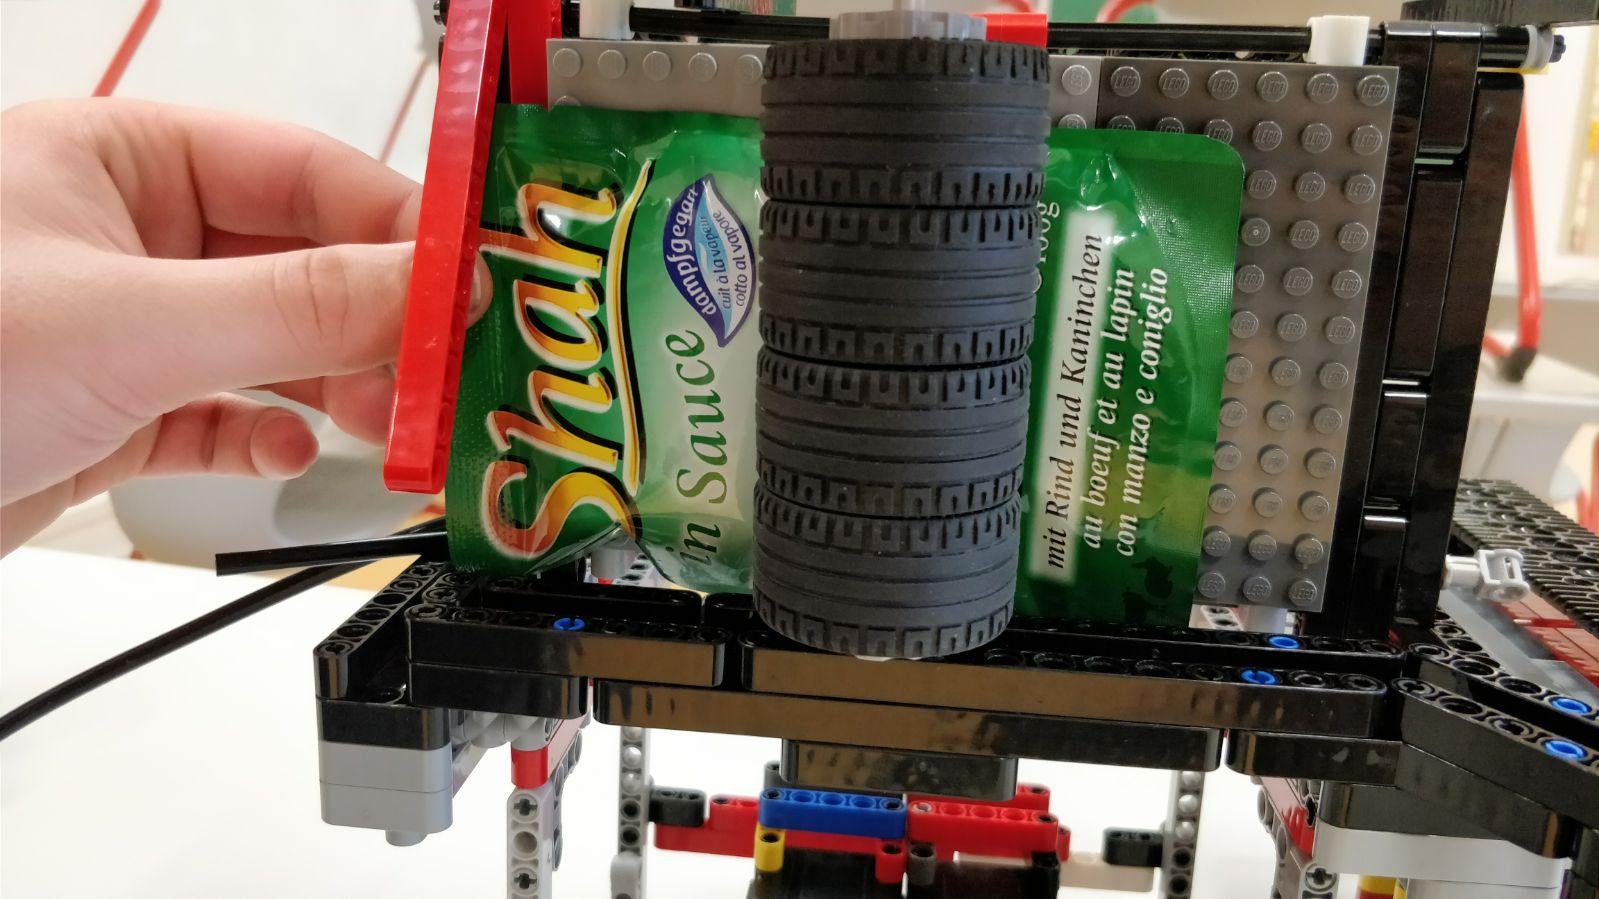
\includegraphics[width=13cm]{Bilder/Ablauf_1_png/Ausquetschen_2}
\caption{Ausquetschen Mitte}
\end{center}
\end{figure}

\begin{figure}[H]
\begin{center}
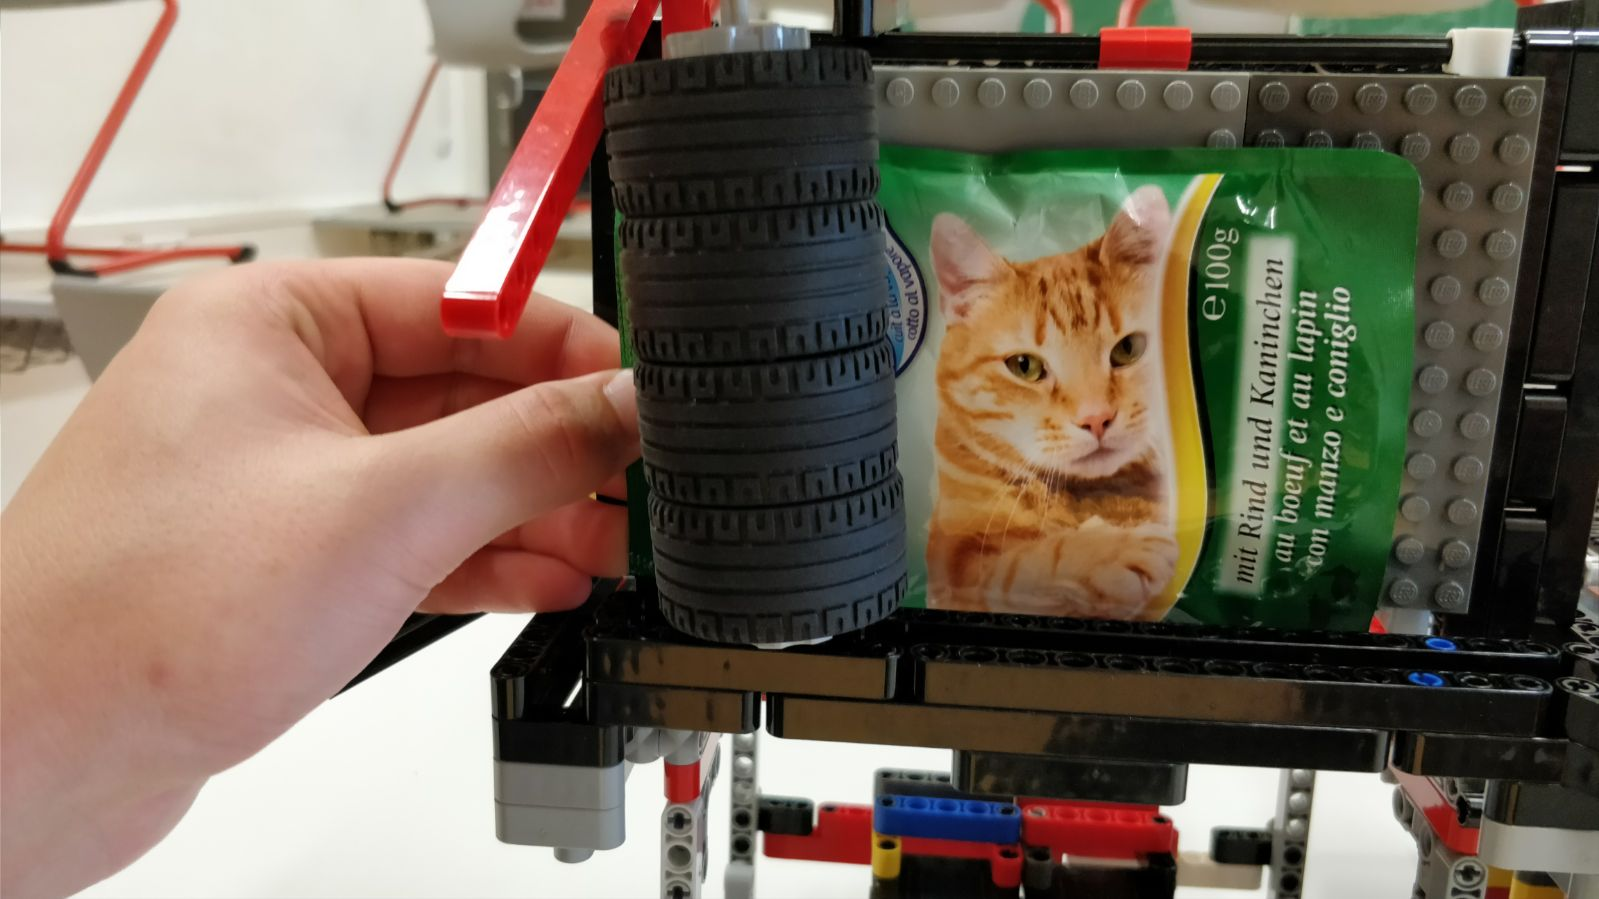
\includegraphics[width=13cm]{Bilder/Ablauf_1_png/Ausquetschen_3}
\caption{Ausquetschen Ende}
\end{center}
\end{figure}
\newpage
\paragraph{Entsorgen}$~~$\\ 

Nach dem Auspressen wird die leere Packung durch die Rückklappe in einen Luftdichten Container geworfen. Die Klappe wird durch zwei Stifte gehalten und lässt sich durch ein Scharnier nach hinten klappen. 

\begin{figure}[H]
\begin{center}
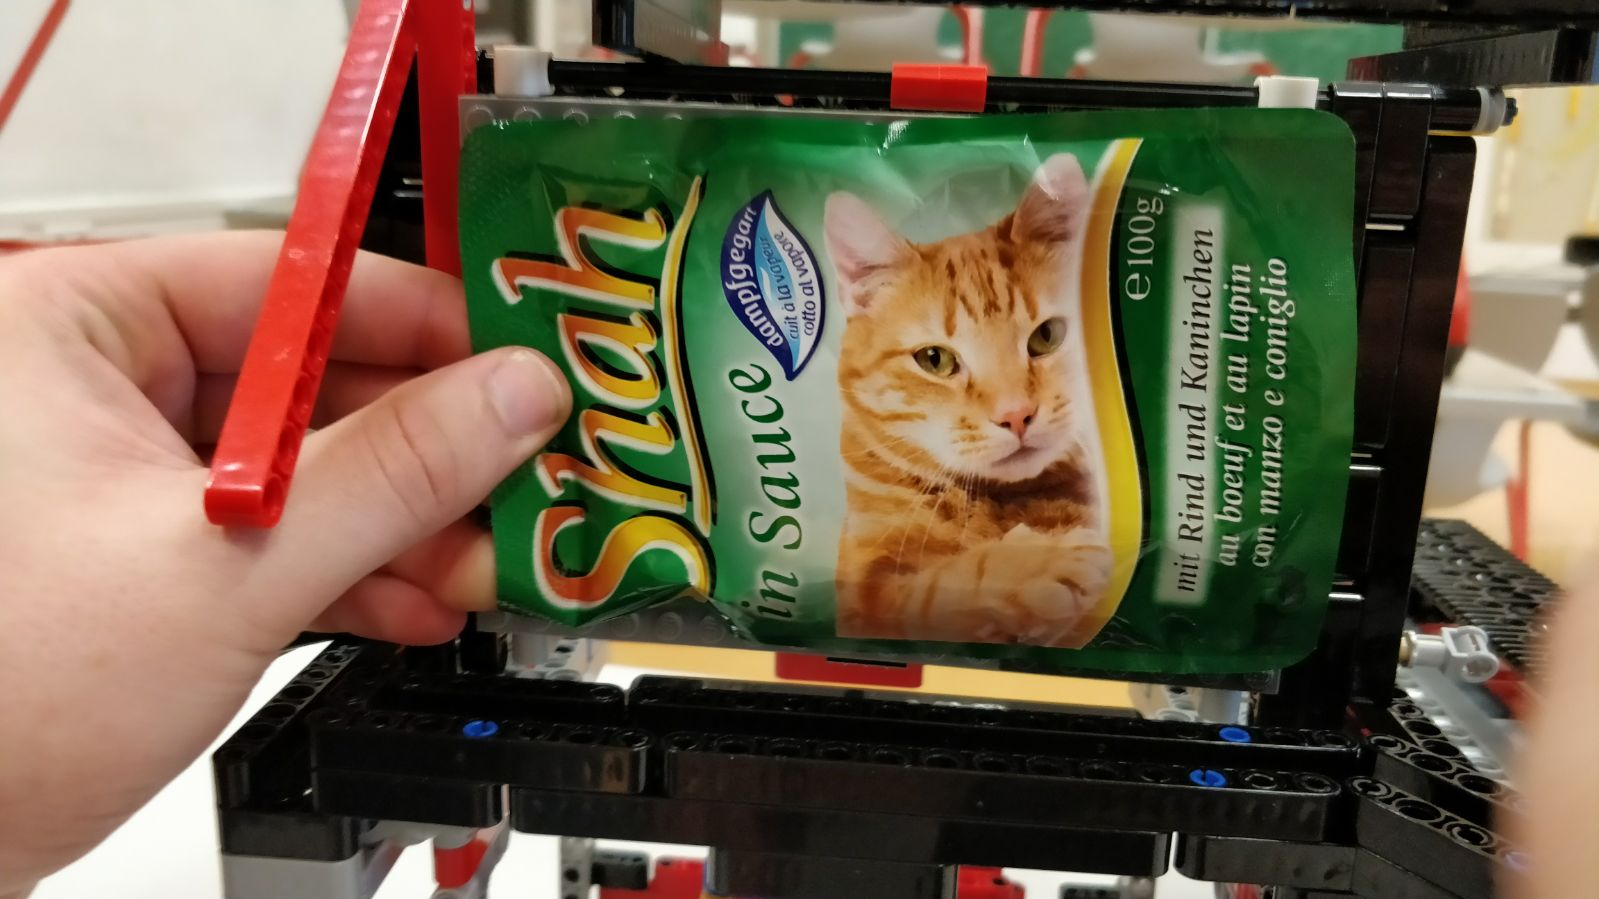
\includegraphics[width=13cm]{Bilder/Ablauf_1_png/Auswurf_1}
\caption{Auswurf Beginn}
\end{center}
\end{figure}

Hier im Bild sieht man den Stift der ein vorzeitiges nach Hinten klappen verhindert

\begin{figure}[H]
\begin{center}
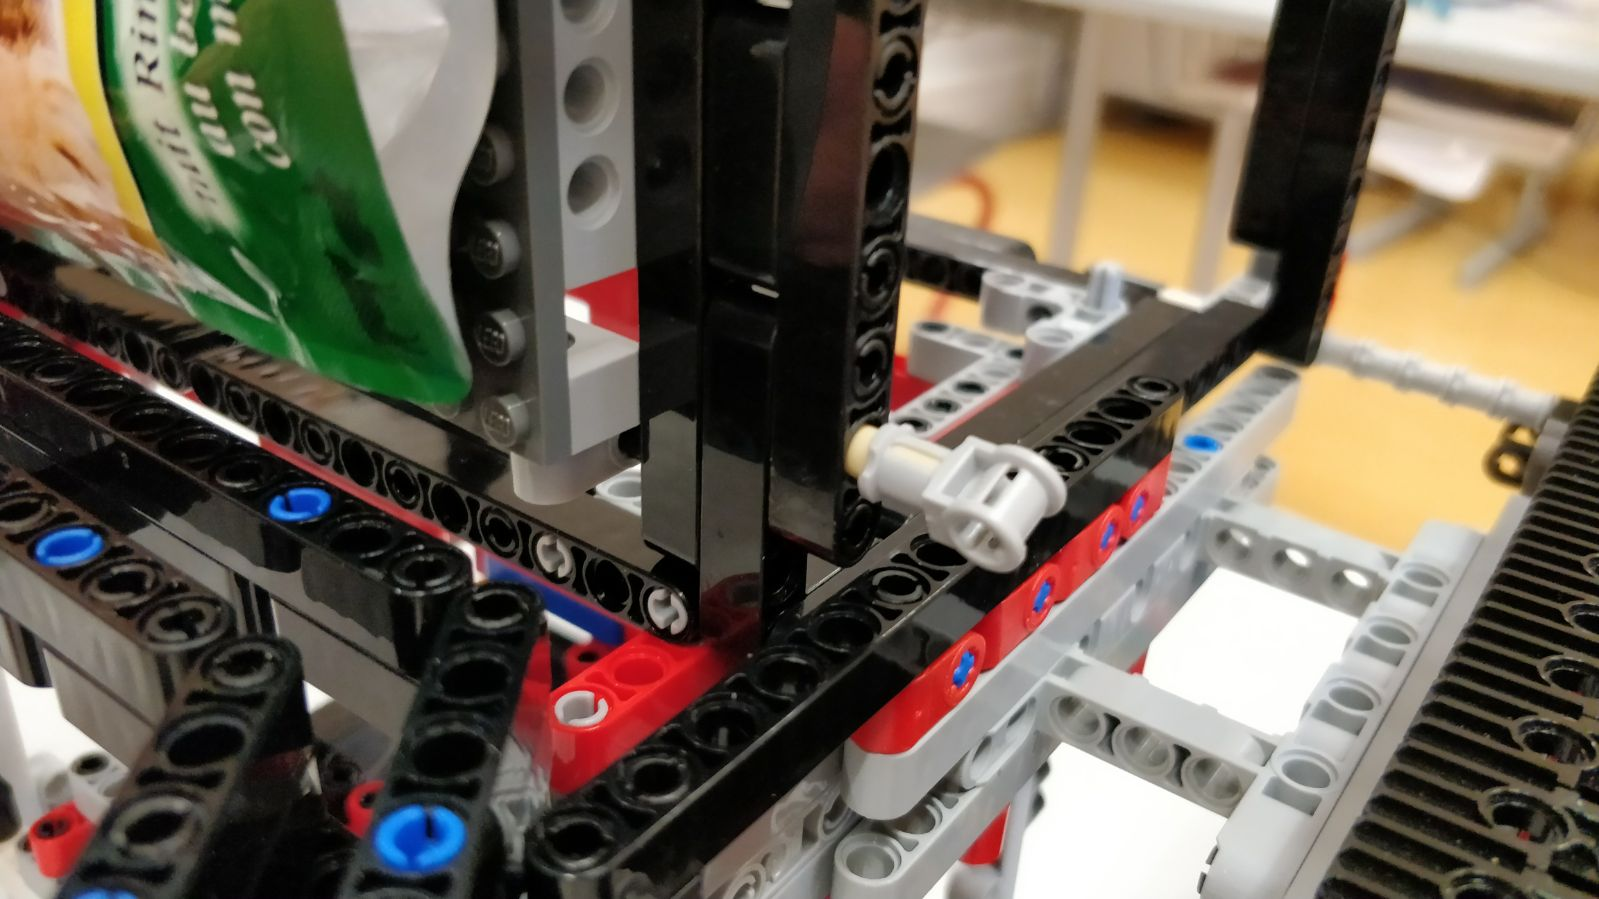
\includegraphics[width=13cm]{Bilder/Ablauf_1_png/Auswurf_2}
\caption{Bolzen drinnen}
\end{center}
\end{figure}

Hier im Bild wurde der Stift entfernt 

\begin{figure}[H]
\begin{center}
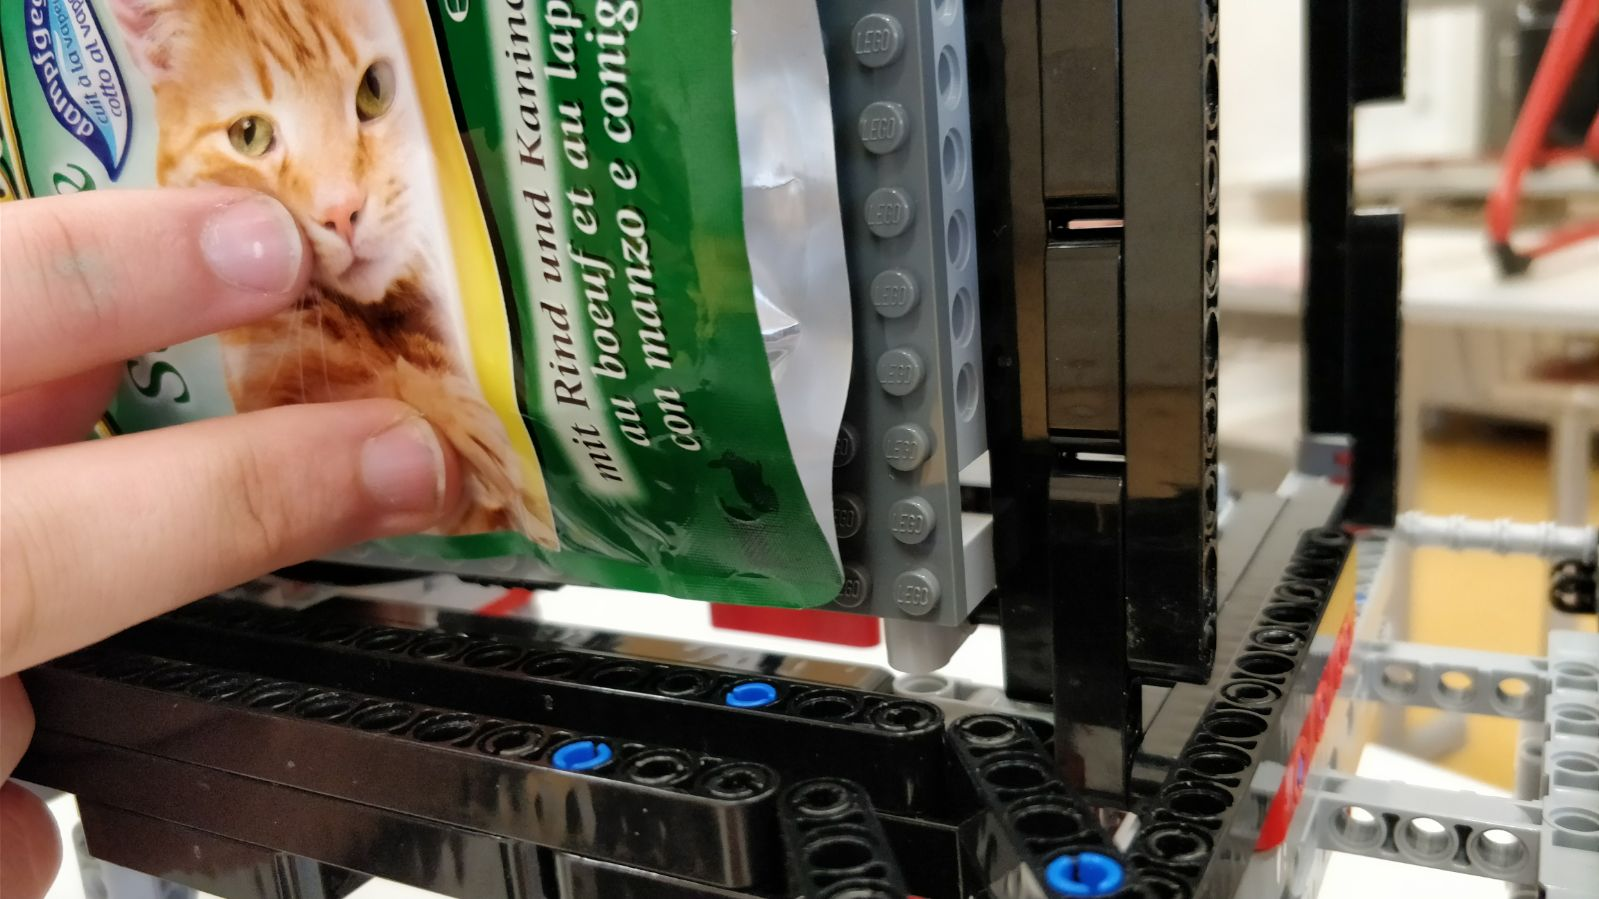
\includegraphics[width=13cm]{Bilder/Ablauf_1_png/Auswurf_3}
\caption{Bolzen entfernen}
\end{center}
\end{figure}

Hier im Bild wird demonstriert wie die Magnetzylinder die leere Packung gegen die Klappe drücken, wodurch die Klappe sich öffnet.

\begin{figure}[H]
\begin{center}
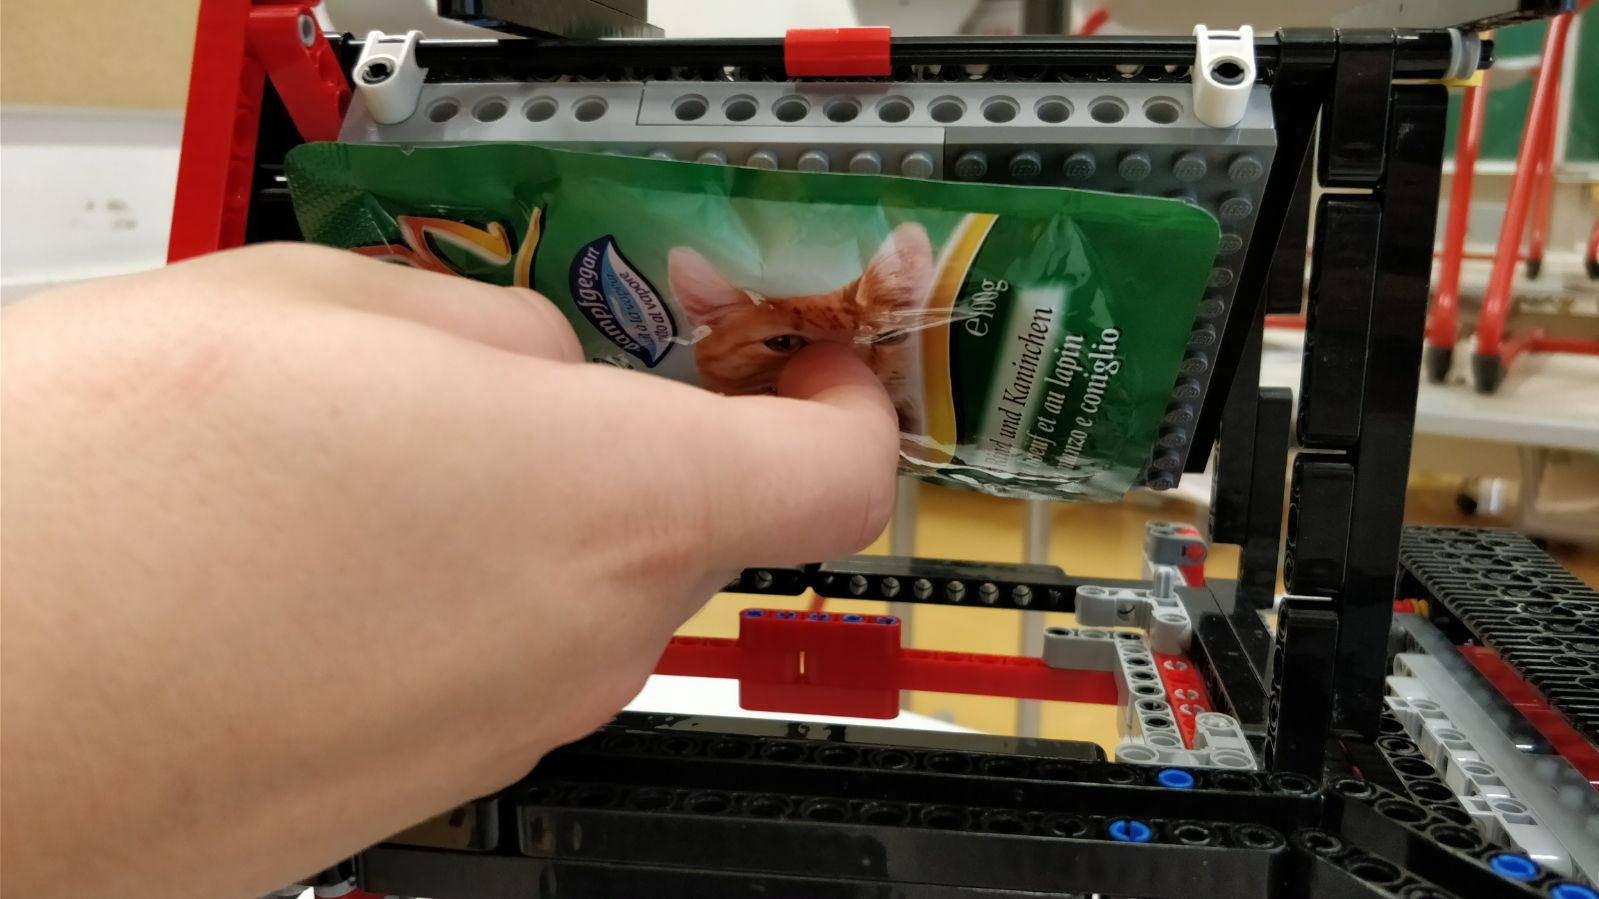
\includegraphics[width=13cm]{Bilder/Ablauf_1_png/Auswurf_4}
\caption{Klappe öffnen}
\end{center}
\end{figure}

\begin{figure}[H]
\begin{center}
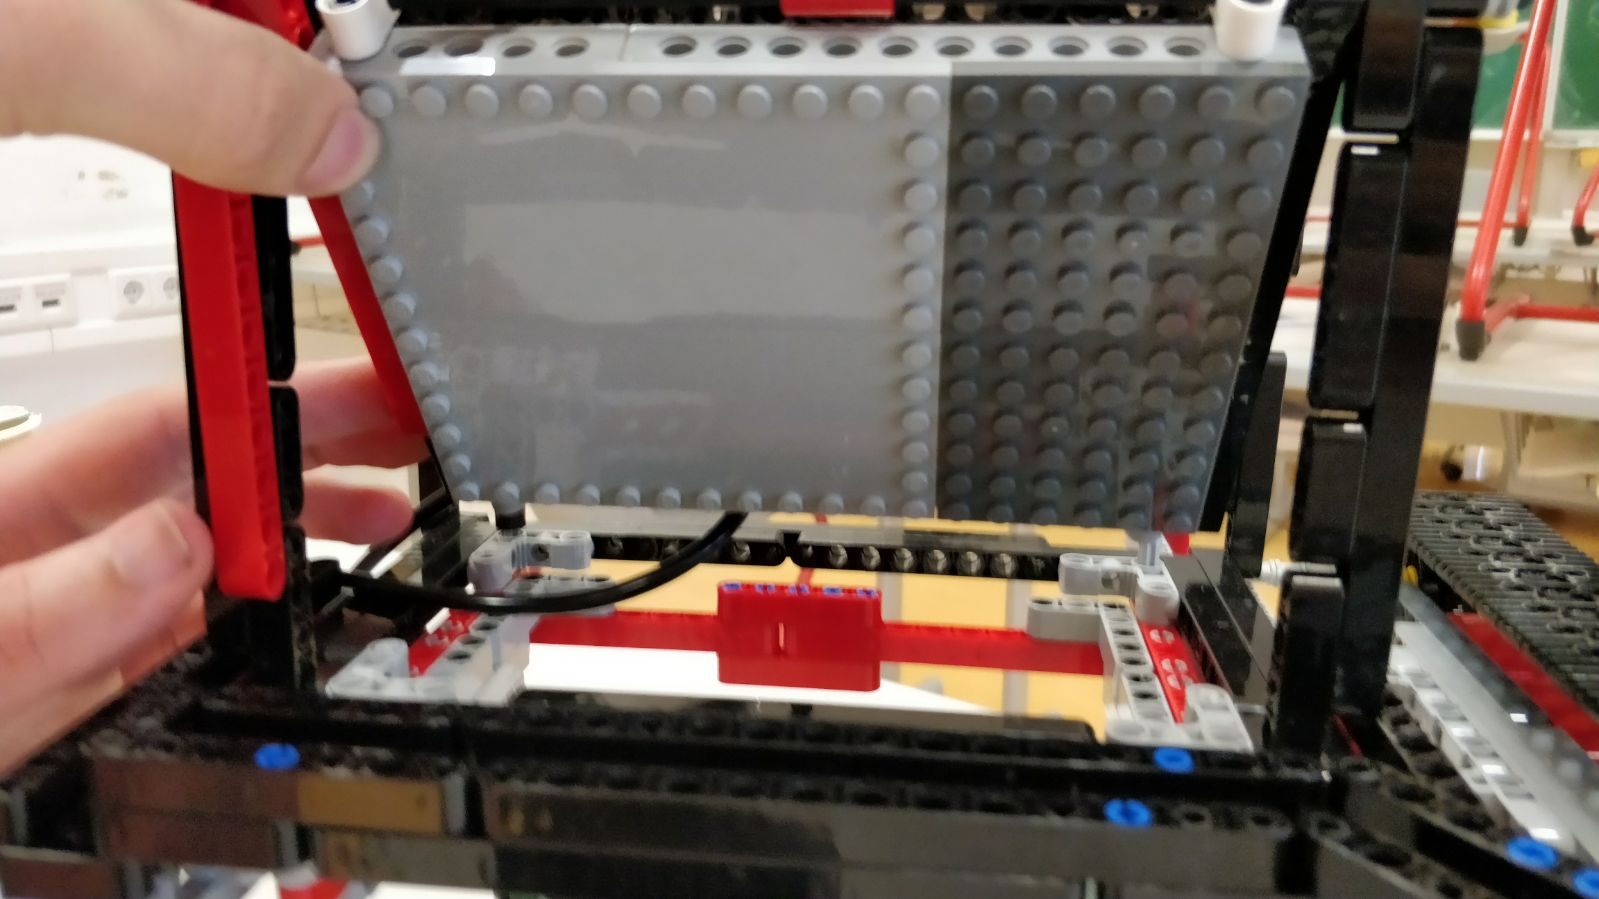
\includegraphics[width=13cm]{Bilder/Ablauf_1_png/Auswurf_5}
\caption{Fertiger Auswurf}
\end{center}
\end{figure}

\paragraph{Füttern}$~~$\\ 

Die Maschine besitzt 5 Futterschüsseln die auf einer drehbaren Platte stehen. Vor dem Füttern wird eine Saubere Platte unter der Stelle, wo später die Packung aufgeschnitten wird, positioniert. Während des Auspressens wird fliegt das Futter in die Futterschüssel. Wenn der Auspressvorgang beendet ist, wird die Futterschüssel an eine Position bewegt, wo die Katze Zugang zum fressen hat.
\newpage


\subsection{Aufbauten und Tests}

In diesem Abteil meiner Diplomarbeit werden verschiedene Tests der obigen Varianten zu sehen sein. \\

\subsubsection{Fütterungsexperiment} 

In diesem Experiment wurde getestet wie lange es Dauert bis eine Packung nur mit Hilfe der Schwerkraft ausläuft. Der Beutel wurde nicht extra erwärmt und wird nur an den beiden unteren Ecken gehalten.

\begin{figure}[H]
   \begin{minipage}[hbt]{.4\linewidth} % [b] => Ausrichtung an \caption
      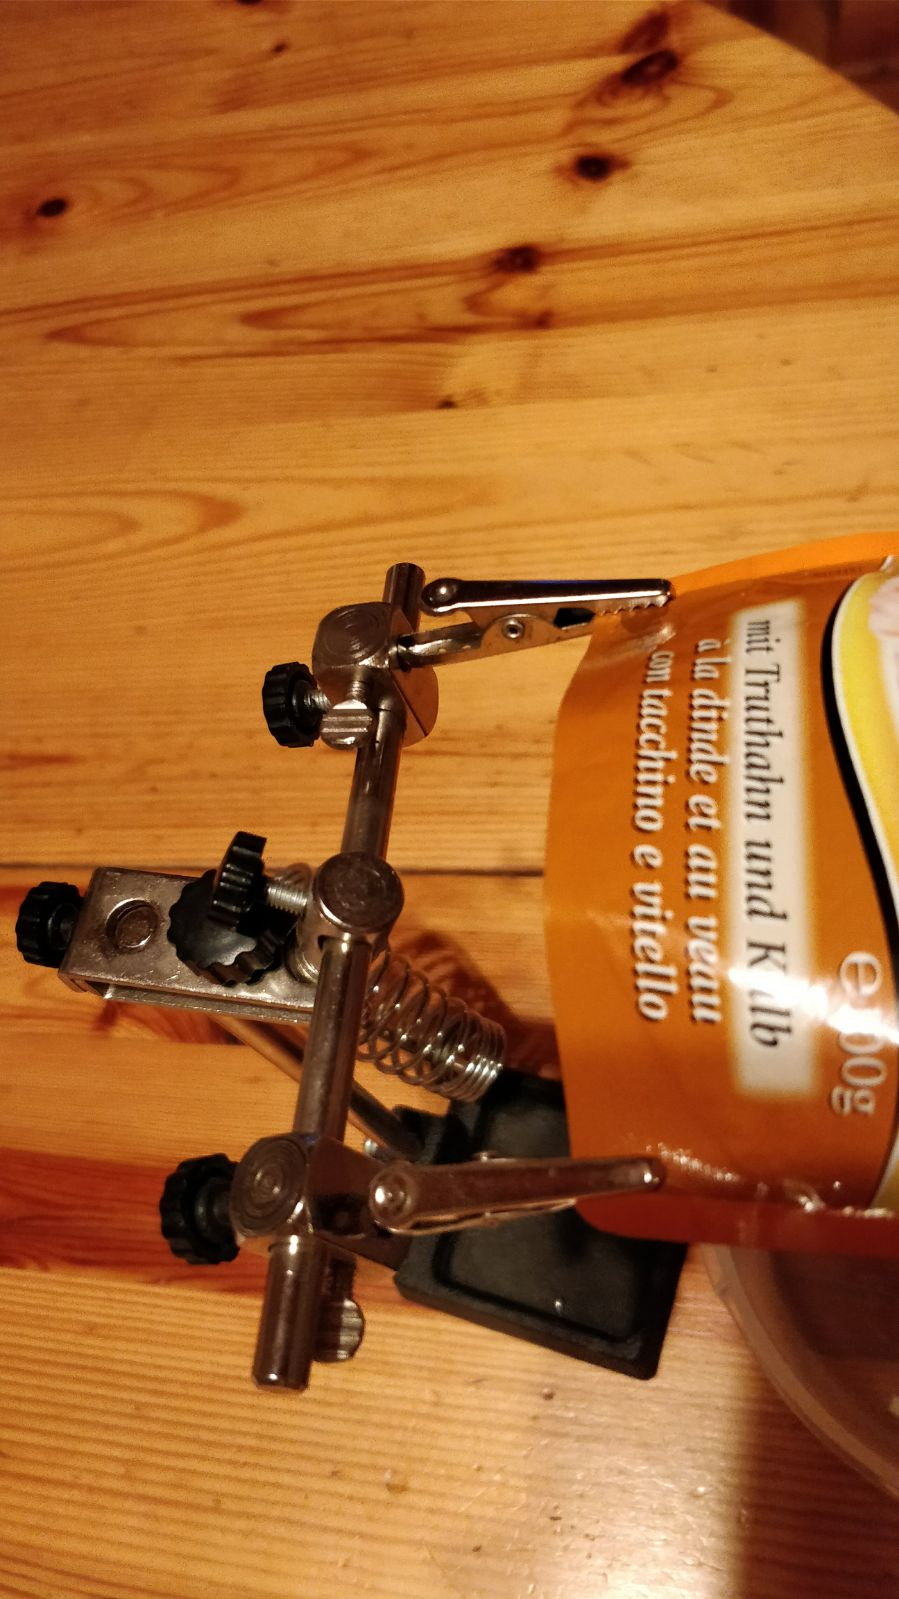
\includegraphics[width=\linewidth]{Bilder/Fuetterungsexperiment/Aufhaengung}
      \caption{Halterung}
   \end{minipage}
   \hspace{.2\linewidth}% Abstand zwischen Bilder
   \begin{minipage}[hbt]{.4\linewidth} % [b] => Ausrichtung an \caption
      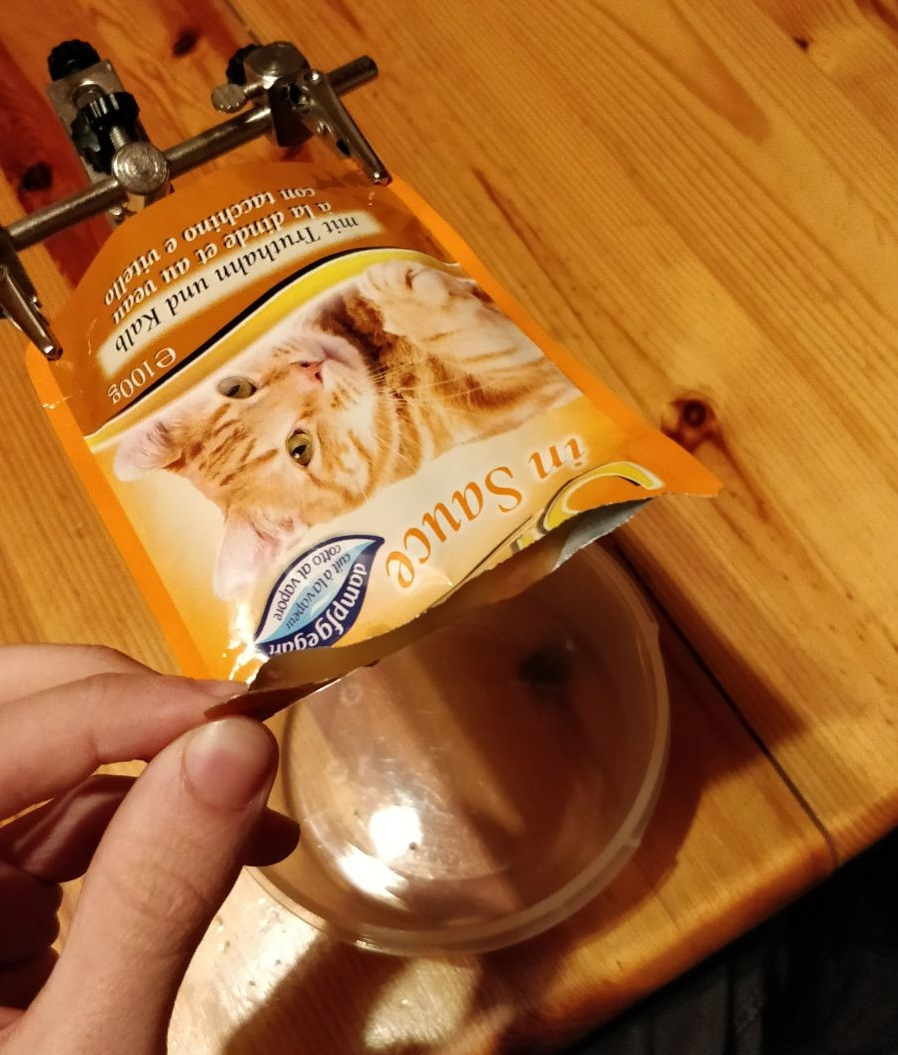
\includegraphics[width=\linewidth]{Bilder/Fuetterungsexperiment/Fuetterungs_Anfang}
      \caption{Fütterungs Anfang}
   \end{minipage}
\end{figure}


\begin{figure}[H]
   \begin{minipage}[hbt]{.3\linewidth} % [b] => Ausrichtung an \caption
      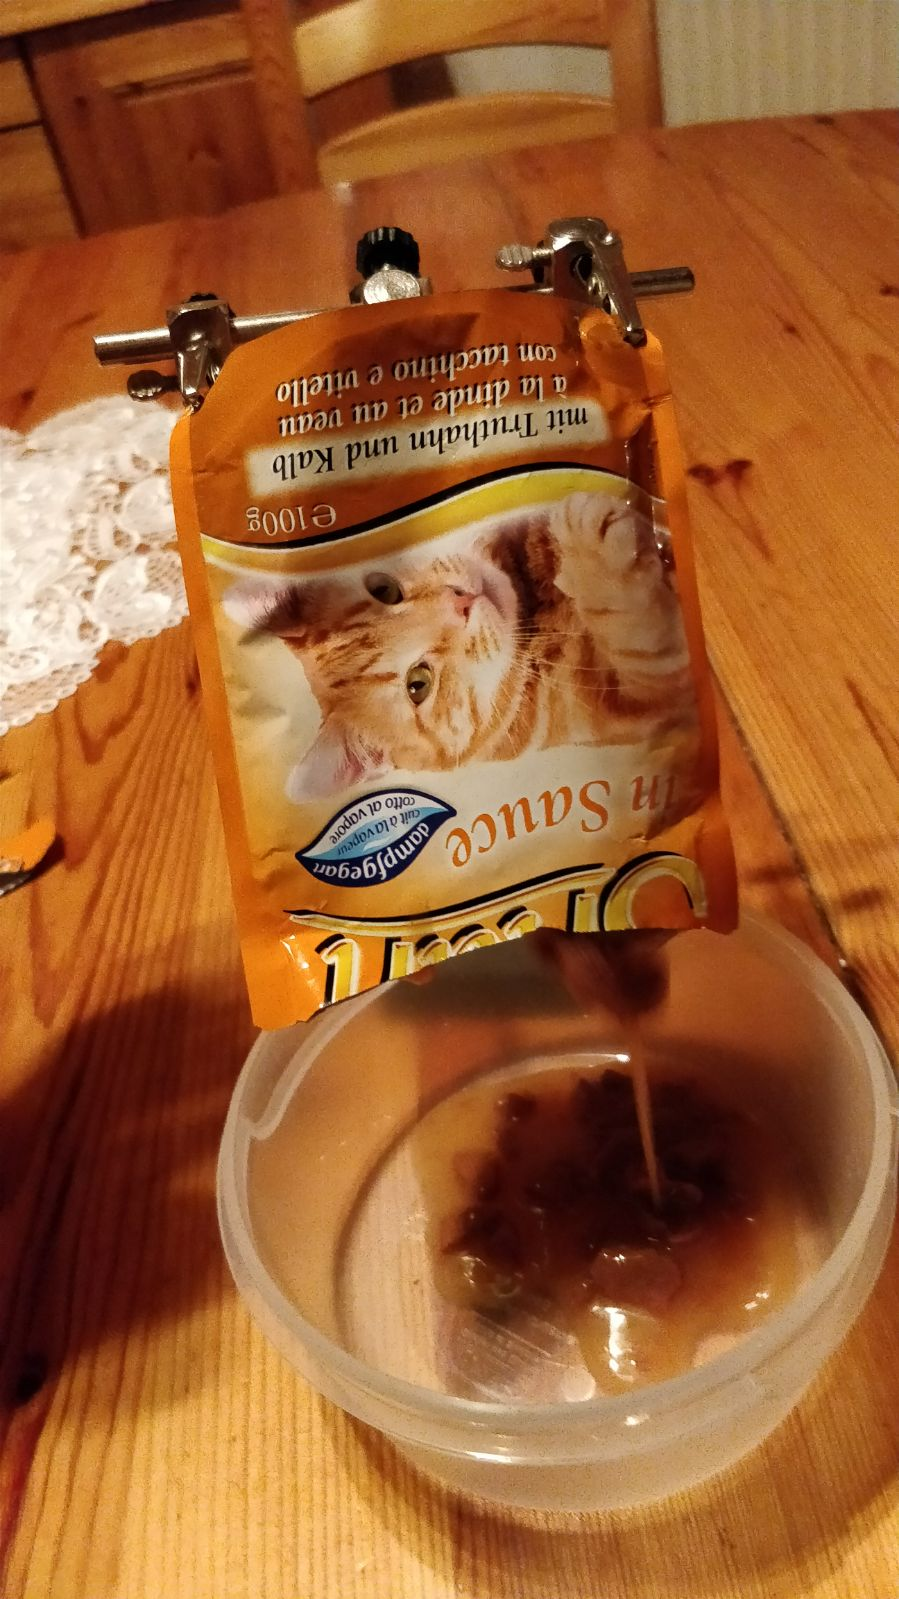
\includegraphics[width=\linewidth]{Bilder/Fuetterungsexperiment/Fuetterungs_Mitte}
      \caption{Fütterungs Mitte}
   \end{minipage}
   \hspace{.4\linewidth}% Abstand zwischen Bilder
   \begin{minipage}[hbt]{.3\linewidth} % [b] => Ausrichtung an \caption
      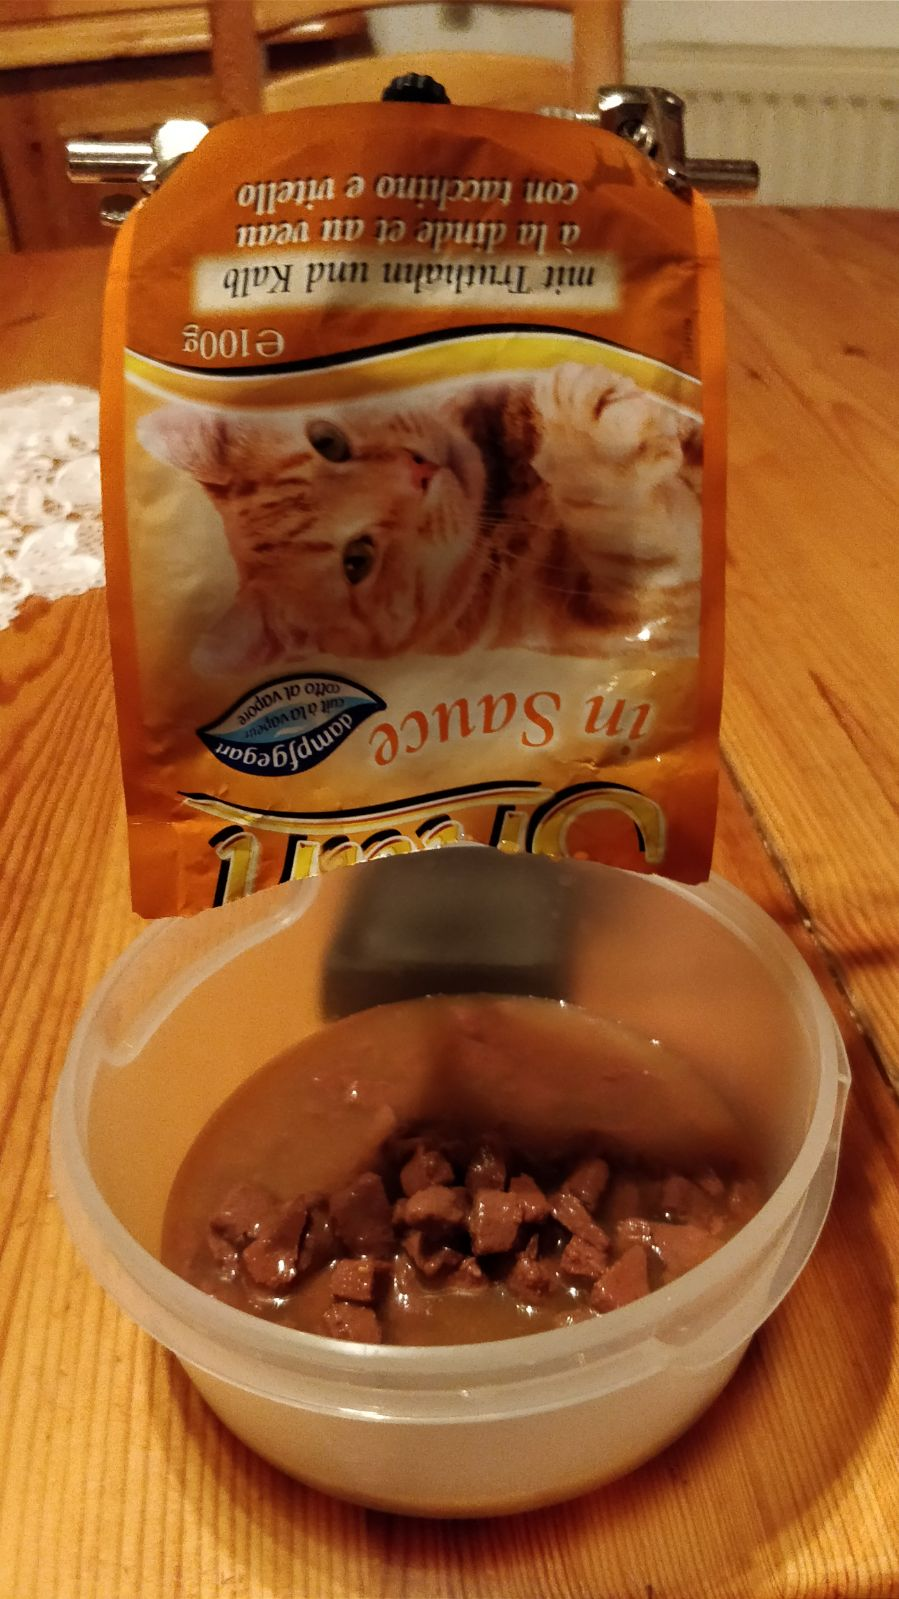
\includegraphics[width=\linewidth]{Bilder/Fuetterungsexperiment/Fuetterungs_Ende}
      \caption{Fütterungs Ende}
   \end{minipage}
\end{figure}

In der Abbildung 20 Fütterungs Ende sieht man das nach 10 Minuten der Inhalte ganz in der Futterschüssel ist, dennoch Tropft es nach.
\newpage
\subsubsection{Schneideversuch 1.Art der 1.Variante}

Schnitt anhand einer praxischen Anwendung dargestellt. Der Beutel wird mithilfe einer Papierschneidemaschine geschnitten.

\begin{figure}[H]
   \begin{minipage}[hbt]{.3\linewidth} % [b] => Ausrichtung an \caption
      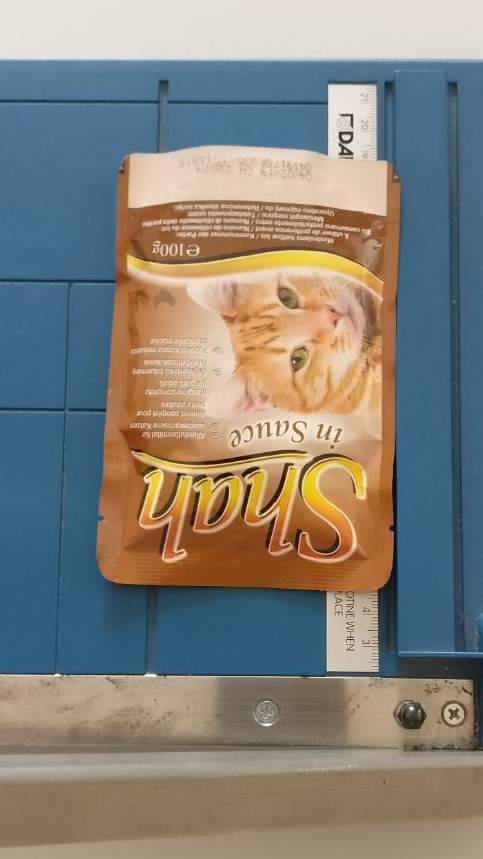
\includegraphics[width=\linewidth]{Bilder/Schneideversuch_1.Art/Einlegen}
      \caption{Einlegen}
   \end{minipage}
   \hspace{.2\linewidth}% Abstand zwischen Bilder
   \begin{minipage}[hbt]{.5\linewidth} % [b] => Ausrichtung an \caption
      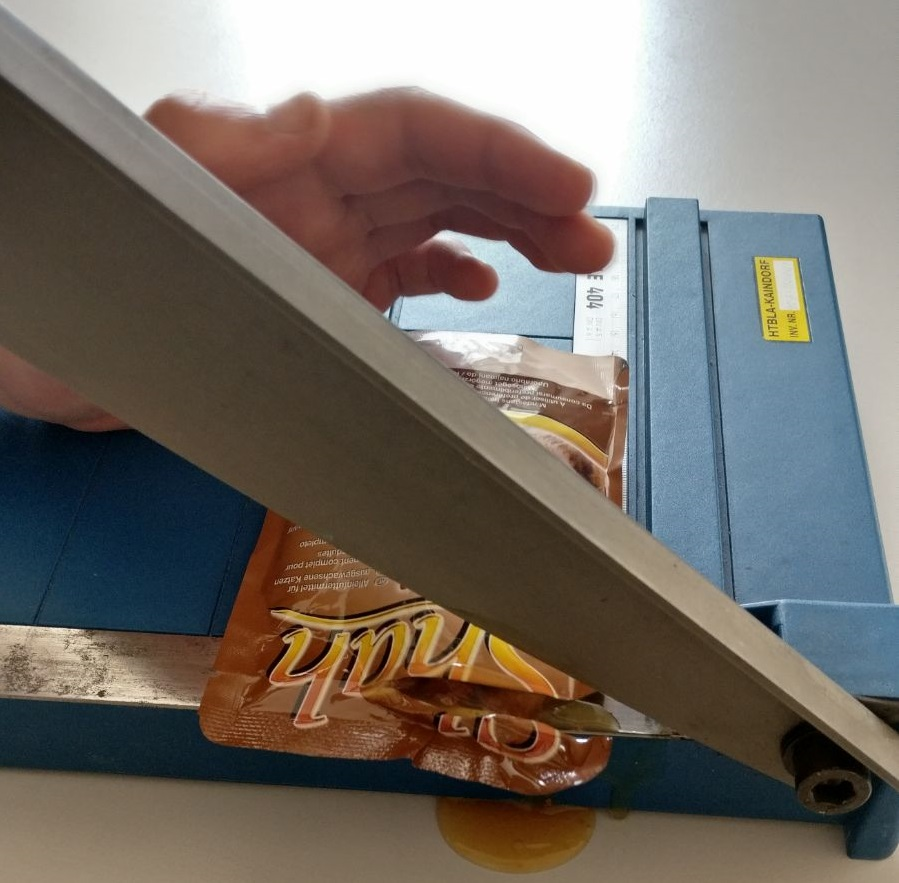
\includegraphics[width=\linewidth]{Bilder/Schneideversuch_1.Art/Anfangsschnitt}
      \caption{Anfangsschnitt}
   \end{minipage}
\end{figure}

\begin{figure}[H]
\begin{center}
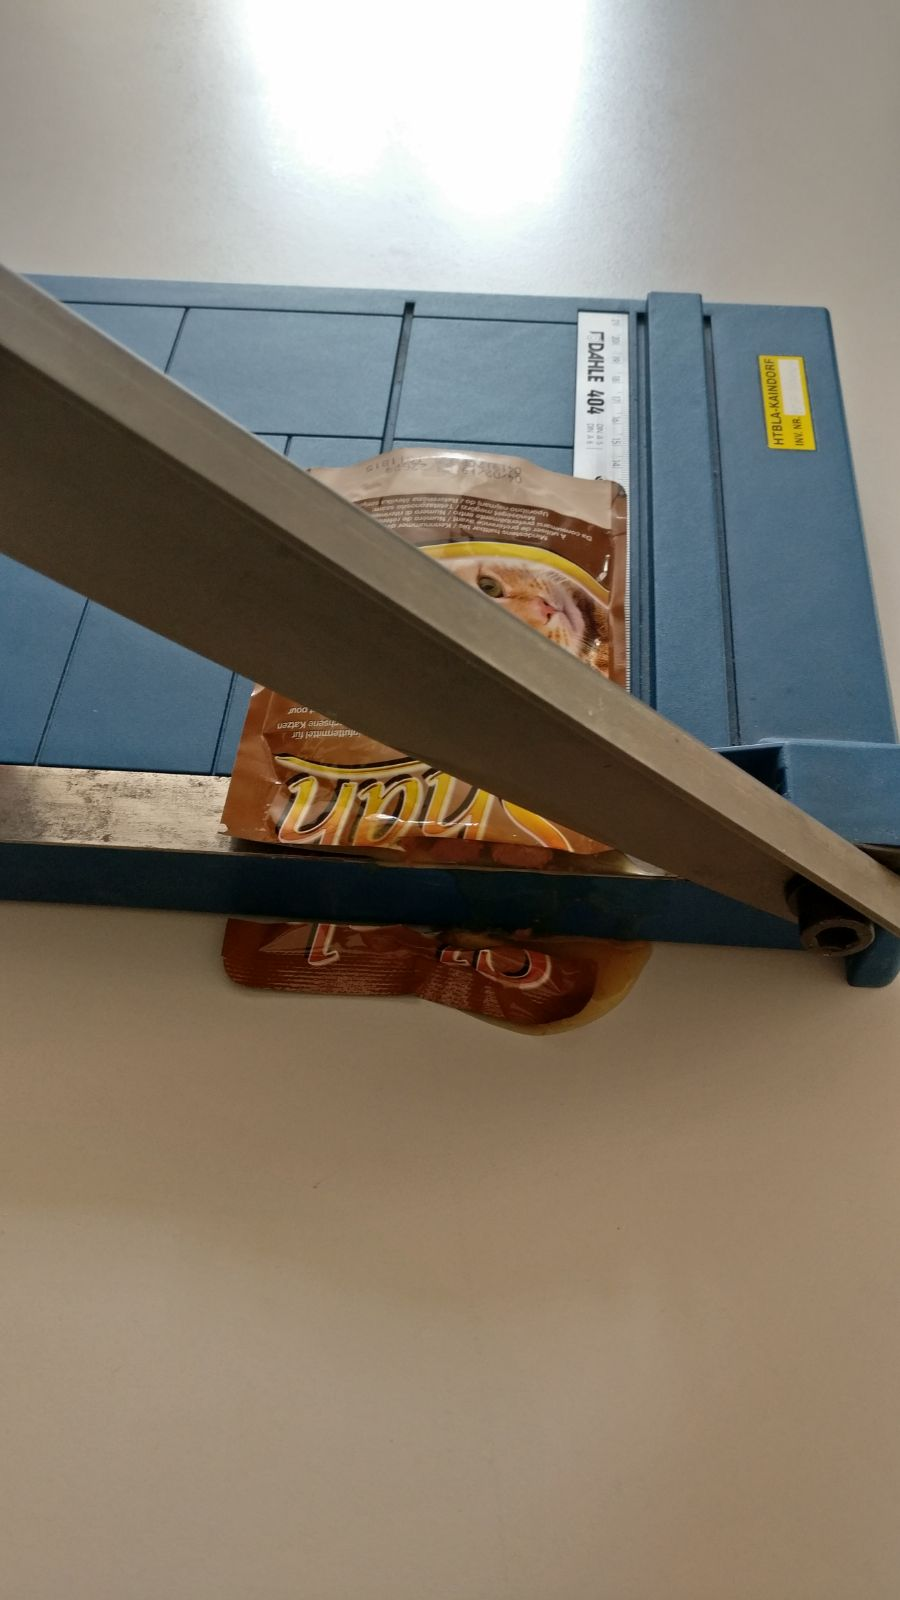
\includegraphics[width=7cm]{Bilder/Schneideversuch_1.Art/Endschnitt}
\caption{Endschnitt}
\end{center}
\end{figure}
\newpage
\subsubsection{Schneideversuch 2.Art der 1.Variante}

Mit einem Metallwerkzeug mit Wellenschliffartiger Kante wird der Futterbeutel entlang der Oberseite aufgeschnitten. Um die Packung vollständig geöffnet zu haben, mussten mehrere Schnitte verwendet werden.\\

\begin{figure}[H]
   \begin{minipage}[hbt]{.3\linewidth} % [b] => Ausrichtung an \caption
      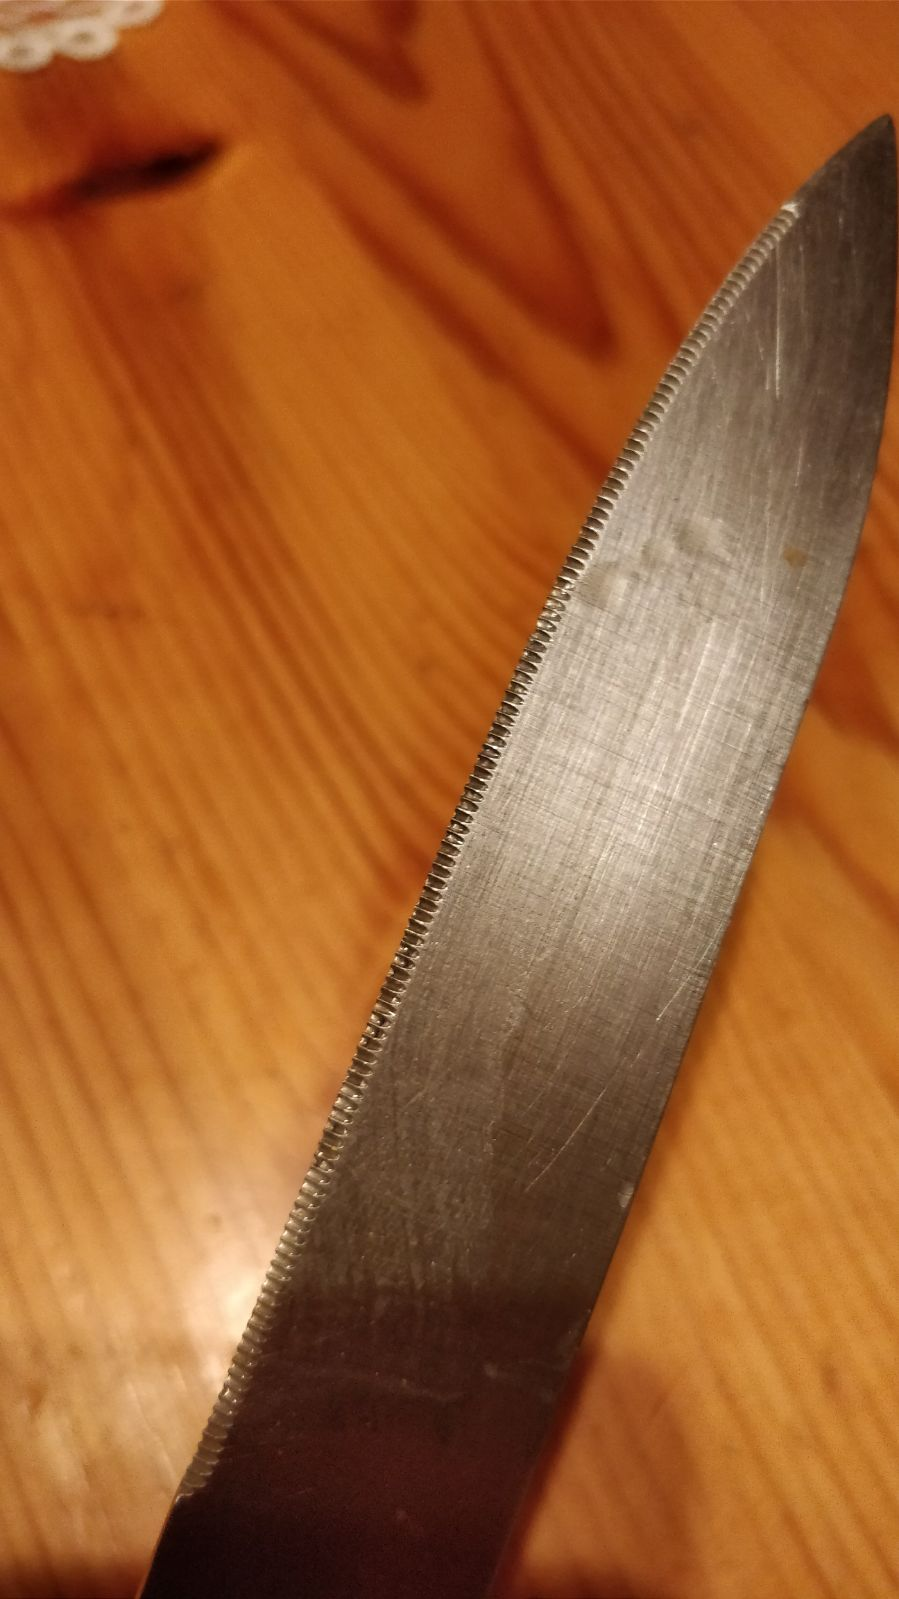
\includegraphics[width=\linewidth]{Bilder/Schneideversuch_2.Art/Schneidemittel}
      \caption{Schneidemittel}
   \end{minipage}
   \hspace{.4\linewidth}% Abstand zwischen Bilder
   \begin{minipage}[hbt]{.3\linewidth} % [b] => Ausrichtung an \caption
      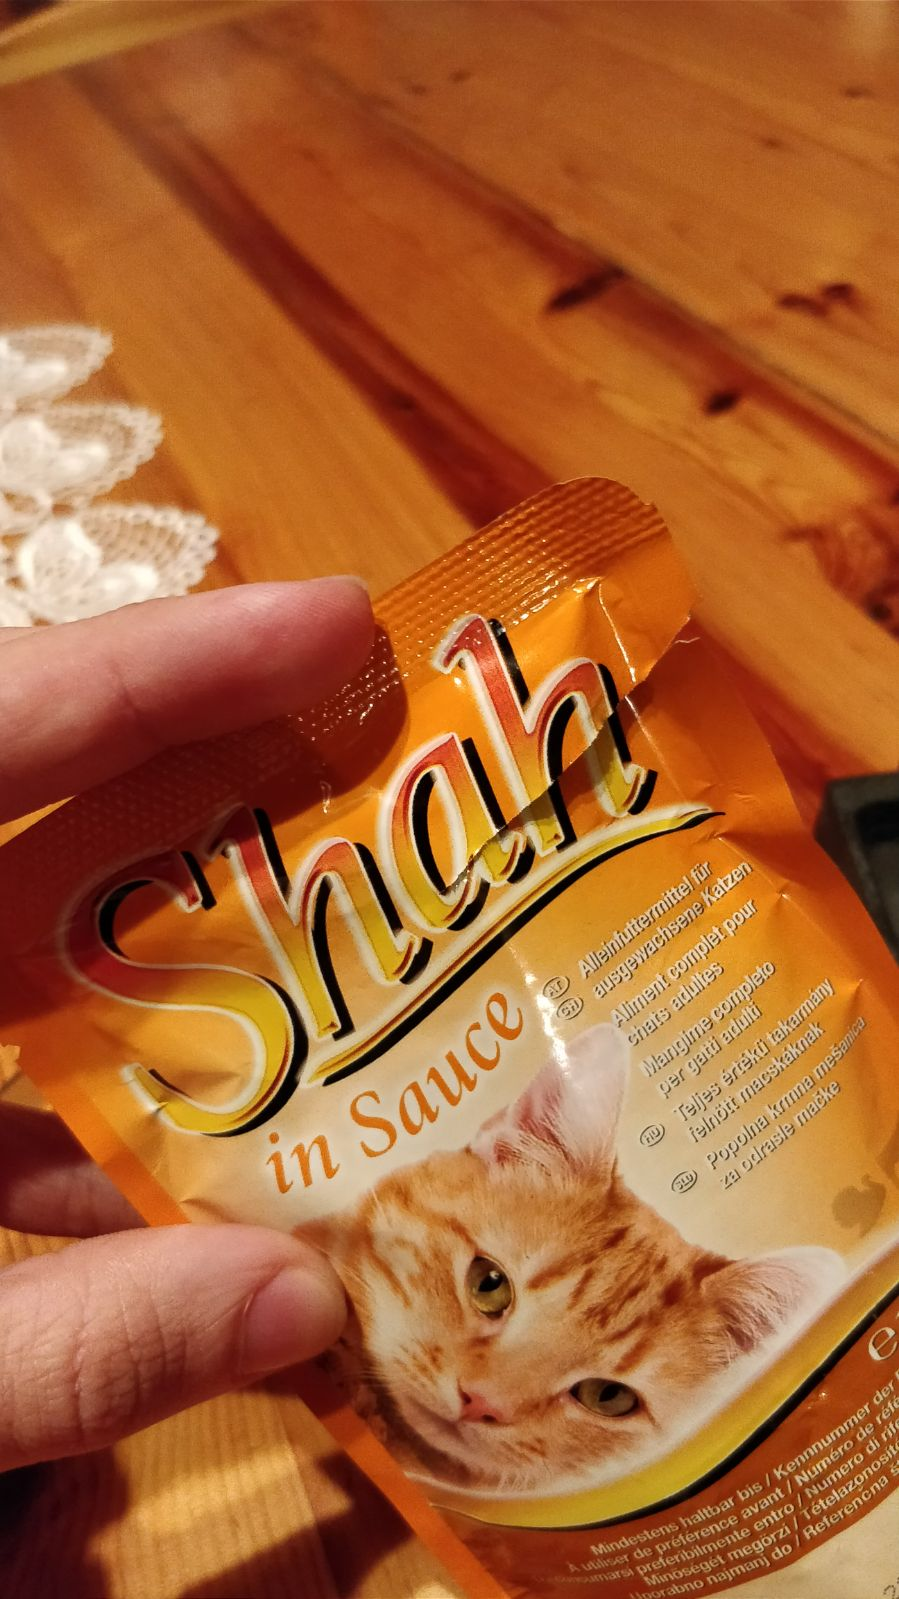
\includegraphics[width=\linewidth]{Bilder/Schneideversuch_2.Art/Anfangsschnitt}
      \caption{Anfangsschnitt 2.Art}
      \label{Nach 3 Schnitten}
   \end{minipage}
\end{figure}

In der Abbildung 25: Anfangschnitt 2.Art erkennt man wie offen die Packung nach 3 Schnitten ist.

\begin{figure}[H]
   \begin{minipage}[hbt]{.4\linewidth} % [b] => Ausrichtung an \caption
      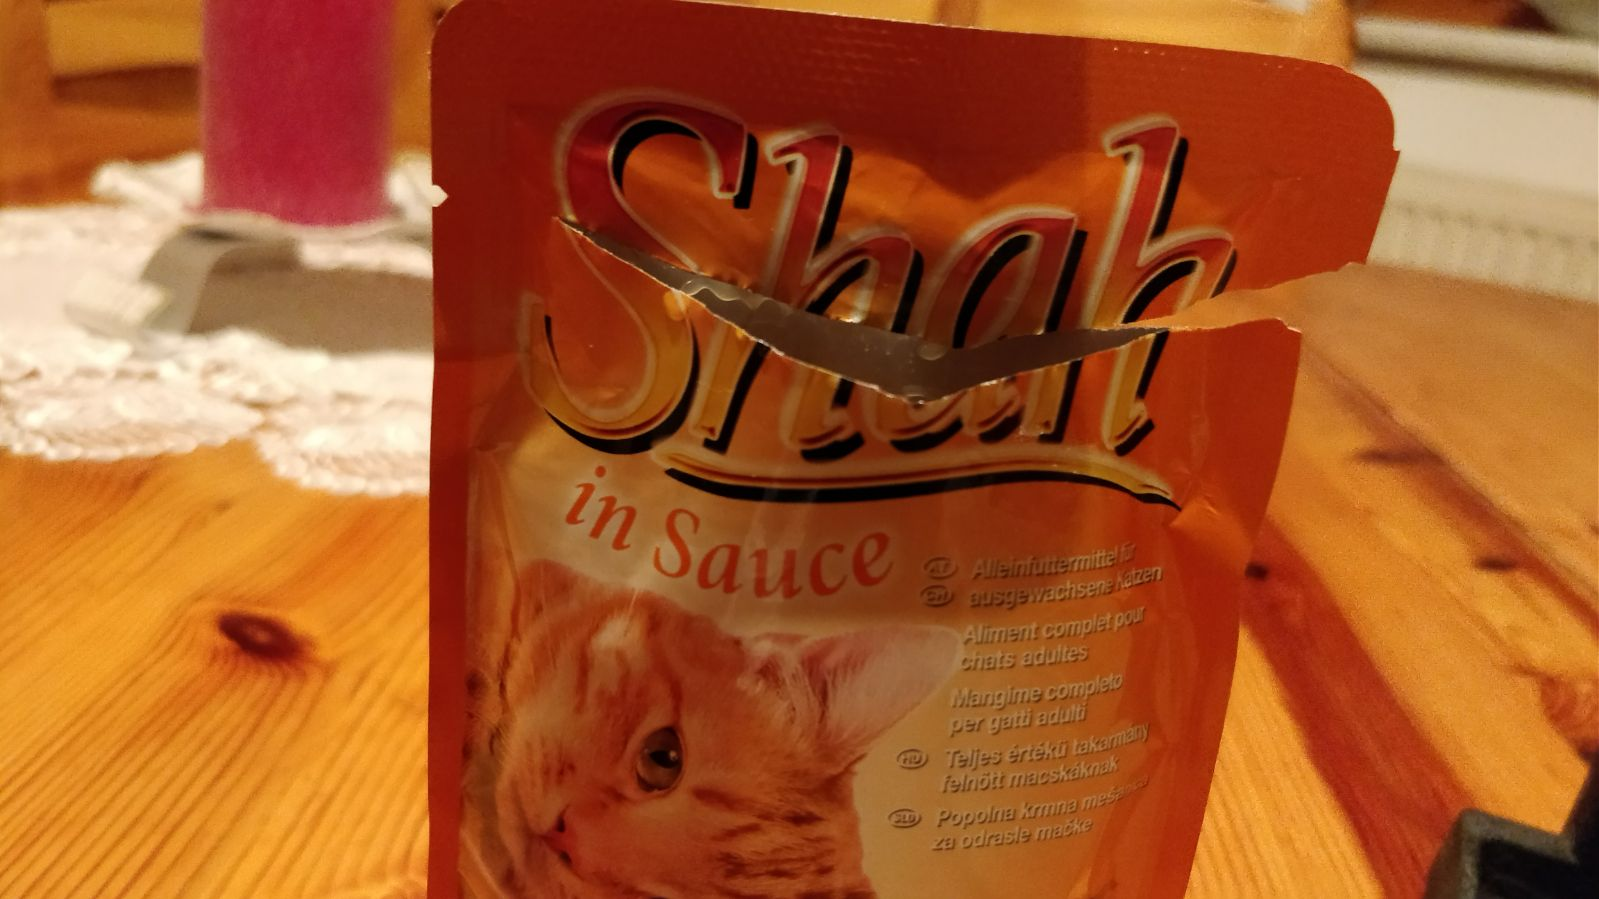
\includegraphics[width=\linewidth]{Bilder/Schneideversuch_2.Art/Mittelschnitt}
      \caption{Mittelschnitt 2.Art}
      \label{Nach 6 Schnitten}
   \end{minipage}
   \hspace{.2\linewidth}% Abstand zwischen Bilder
   \begin{minipage}[hbt]{.4\linewidth} % [b] => Ausrichtung an \caption
      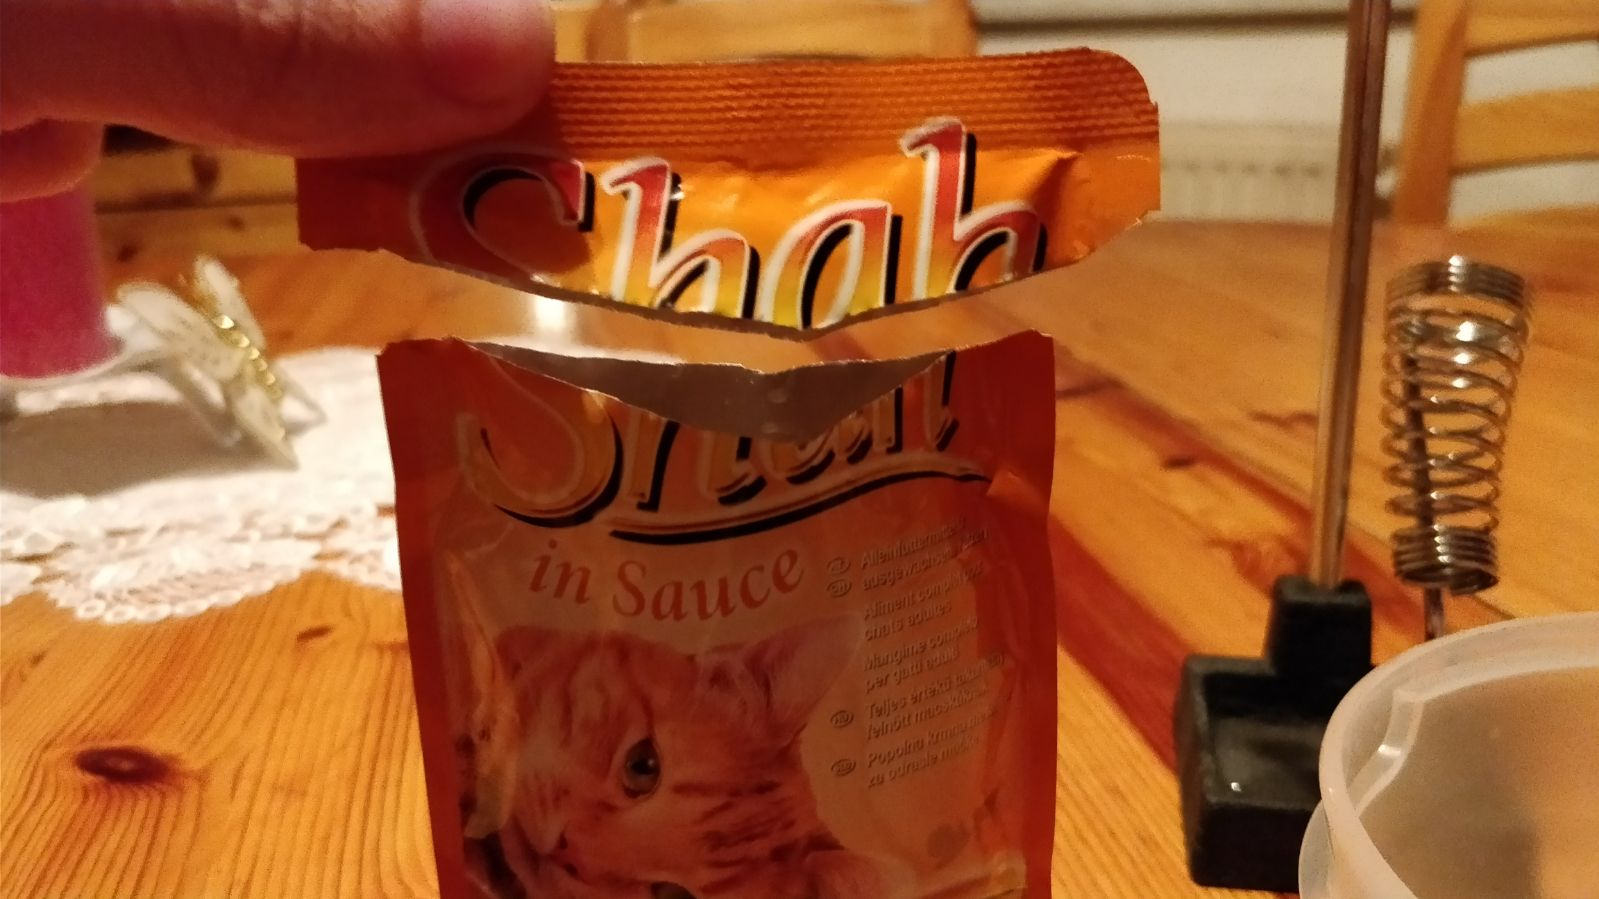
\includegraphics[width=\linewidth]{Bilder/Schneideversuch_2.Art/Endschnitt}
      \caption{Endschnitt 2.Art}
      \label{Nach 9 Schnitten}
   \end{minipage}
\end{figure}
In der Abbildung 26: Mittelschnitt 2.Art erkennt man wie offen die Packung nach 6 Schnitten ist.\\

In der Abbildung 27: Endschnitt 2.Art wurde die Packung nach 9 Schnitten vollständig geöffnet.

\subsection{Vergleich der Varianten}
\subsection{Konstruktion der Wahlvariante und Details}
\subsection{Berechnung und Dimensionierung}
\subsection{Simulation}
\subsection{Bedienung und Wartung}
\subsection{Selbstkritische Analyse und Ausblick}


\end{document}
